%definira klasu dokumenta 
\documentclass[12pt]{report} 

%prostor izmedu naredbi \documentclass i \begin{document} se zove uvod. U njemu se nalaze naredbe koje se odnose na cijeli dokument

%osnovni LaTex ne može riješiti sve probleme, pa se koriste različiti paketi koji olakšavaju izradu željenog dokumenta
\usepackage[croatian]{babel} 
\usepackage{amssymb}
\usepackage{amsmath}
\usepackage{txfonts}
\usepackage{mathdots}
\usepackage{titlesec}
\usepackage{array}
\usepackage{lastpage}
\usepackage{etoolbox}
\usepackage{tabularray}
\usepackage{color, colortbl}
\usepackage{adjustbox}
\usepackage{geometry}
\usepackage[classicReIm]{kpfonts}
\usepackage{hyperref}
\usepackage{fancyhdr}

\usepackage{float}
\usepackage{setspace}
\restylefloat{table}


\patchcmd{\chapter}{\thispagestyle{plain}}{\thispagestyle{fancy}}{}{} %redefiniranje stila stranice u paketu fancyhdr

%oblik naslova poglavlja
\titleformat{\chapter}{\normalfont\huge\bfseries}{\thechapter.}{20pt}{\Huge}
\titlespacing{\chapter}{0pt}{0pt}{40pt}


\linespread{1.3} %razmak između redaka

\geometry{a4paper, left=1in, top=1in,}  %oblik stranice

\hypersetup{ colorlinks, citecolor=black, filecolor=black, linkcolor=black,	urlcolor=black }   %izgled poveznice


%prored smanjen između redaka u nabrajanjima i popisima
\newenvironment{packed_enum}{
	\begin{enumerate}
		\setlength{\itemsep}{0pt}
		\setlength{\parskip}{0pt}
		\setlength{\parsep}{0pt}
	}{\end{enumerate}}

\newenvironment{packed_item}{
	\begin{itemize}
		\setlength{\itemsep}{0pt}
		\setlength{\parskip}{0pt}
		\setlength{\parsep}{0pt}
	}{\end{itemize}}




%boja za privatni i udaljeni kljuc u tablicama
\definecolor{LightBlue}{rgb}{0.9,0.9,1}
\definecolor{LightGreen}{rgb}{0.9,1,0.9}

%Promjena teksta za dugačke tablice
\DefTblrTemplate{contfoot-text}{normal}{Nastavljeno na idućoj stranici}
\SetTblrTemplate{contfoot-text}{normal}
\DefTblrTemplate{conthead-text}{normal}{(Nastavljeno)}
\SetTblrTemplate{conthead-text}{normal}
\DefTblrTemplate{middlehead,lasthead}{normal}{Nastavljeno od prethodne stranice}
\SetTblrTemplate{middlehead,lasthead}{normal}

%podesavanje zaglavlja i podnožja

\pagestyle{fancy}
\lhead{Programsko inženjerstvo}
\rhead{ConnectiNET}
\lfoot{Eventio}
\cfoot{stranica \thepage/\pageref{LastPage}}
\rfoot{\today}
\renewcommand{\headrulewidth}{0.2pt}
\renewcommand{\footrulewidth}{0.2pt}


\begin{document} 
	
	
	
	\begin{titlepage}
		\begin{center}
			\vspace*{\stretch{1.0}} %u kombinaciji s ostalim \vspace naredbama definira razmak između redaka teksta
			\LARGE Programsko inženjerstvo\\
			\large Ak. god. 2023./2024.\\
			
			\vspace*{\stretch{3.0}}
			
			\huge ConnectiNET\\
			\Large Dokumentacija, Rev. \textit{2}\\
			
			\vspace*{\stretch{12.0}}
			\normalsize
			Grupa: \textit{Eventio}\\
			Voditelj: \textit{Gašpar Haramija}\\
			
			
			\vspace*{\stretch{1.0}}
			Datum predaje: \textit{X. siječanj 2024.}\\
	
			\vspace*{\stretch{4.0}}
			
			Nastavnik: \textit{Nikolina Frid}\\
		
		\end{center}

	
	\end{titlepage}

	
	\tableofcontents


	\chapter{Dnevnik promjena dokumentacije}
		
				
		
		\begin{longtblr}[
				label=none
			]{
				width = \textwidth, 
				colspec={|X[2]|X[13]|X[3]|X[3]|}, 
				rowhead = 1
			}
			\hline
			\textbf{Rev.}	& \textbf{Opis promjene/dodatka} & \textbf{Autori} & \textbf{Datum}\\[3pt] \hline
			0.1 & Napravljen predložak.	& Gašpar Haramija & 24.10.2023. 		\\[3pt] \hline 
			0.2	& Ažuriranje dnevnika sastajanja. & Filip Buhiniček & 26.10.2023. 	\\[3pt] \hline 
			0.3	& Dodavanje općeg UC dijagrama te pojedinačnih UC dijagrama. Dodane reference. & Sandro Boka & 30.10.2023. 	\\[3pt] \hline 
			0.4	& Izrada i dopuna funkcionalnih zahtjeva.\newline Dodane reference. & Mateo Grdić & 31.10.2023. 	\\[3pt] \hline 
			0.5 & Dodani tekstualni opisi obrazaca uporabe & Marko Srsic, Jakov Šarolić & 31.10.2023. \\[3pt] \hline 
			0.6 & Dopisan opis projekta te ažuriran dnevnik promjena dokumentacije & Filip Buhiniček, Gašpar Haramija & 01.11.2023. \\[3pt] \hline 
			0.7 & Sekvencijski dijagrami & Gašpar Haramija & 02.11.2023. \\[3pt] \hline 
			0.8.1 & Prva verzija dijagrama razreda & Sandro Boka, Marko Sršić & 03.11.2023. \\[3pt] \hline 
			0.8.2 & Nastavak i ažuriranje dijagrama razreda & Sandro Boka, Marko Sršić & 15.11.2023. \\[3pt] \hline 
			0.9 & Ažuriranje dokumentacije, brisanje template dijelova & Marko Sršić & 16.11.2023. \\[3pt] \hline 
			
			\textbf{1.0} & Verzija samo s bitnim dijelovima za 1. ciklus & Gašpar Haramija & 17.11.2023. \\[3pt] \hline 
			
			1.1 & Ažuriranje obrazaca uporabe prema uputama iz 1. revizije & Sandro Boka, Marko Sršić & 9.12.2023. \\[3pt] \hline 
			1.2 & Brisanje template dijelova  & Marko Sršić & 18.12.2023. \\[3pt] \hline 
			1.3 & Dijagram stanja & Marko Sršić & 19.12.2023. \\[3pt] \hline 
			1.4 & Dijagram aktivnosti & Marko Sršić & 20.12.2023. \\[3pt] \hline
			1.5.1 & Razni ispravci (funkcionalni zahtjevi, obrasci uporabe, arhitektura i dizajn sustava, itd.) & Marko Sršić & 4.1.2024. \\[3pt] \hline 
			1.5.2 & Ažuriranje dnevnika sastajanja, tablice aktivnosti & Marko Sršić & 11.1.2024. \\[3pt] \hline 
			1.6 & Dijagram komponenti, dijagram razmještaja & Gašpar Haramija & 13.1.2024. \\[3pt] \hline 
			1.7 & Korištene tehnologije, ispitivanje komponenti/sustava & Gašpar Haramija & 14.1.2024. \\[3pt] \hline 
			1.8 & Upute za puštanje u pogon & Gašpar Haramija & 15.1.2024. \\[3pt] \hline 
			1.9 & Dijagrami pregleda promjena, zaključak i budući rad & Gašpar Haramija & 15.1.2024. \\[3pt] \hline 
			\textbf{2.0} & Konačni tekst predloška dokumentacije  & Gašpar Haramija, Marko Sršić & 18.1.2024. \\[3pt] \hline 
		\end{longtblr}
	
	\chapter{Opis projektnog zadatka}
		
		\textbf{\textit{dio 1. revizije}}\\
		
		Cilj ovog projekta je razviti programsku podršku za stvaranje web aplikacije "Eventio", koja će korisnicima omogućiti stvaranje, oglašavanje i sudjelovanje na različitim događanjima. Ova inovativna web aplikacija će korisnicima omogućiti lakši pristup društevnim događanjima koja odgovaraju njihovim interesima te olakšati organizaciju i promociju istih.
		
		Postoje mnoge društvene platforme koje već imaju razvijene mreže korisnika i nude vlastite implementacije sličnih rješenja za događanja. Međutim, ono što "Eventio" čini drugačijim jest njegov pristup. Dok druga rješenja ovise o korisnicima koji stvaraju različite grupe i objavljuju događanja na koje se korisnici prijavljuju ili postaju članovi tih grupa (primjer toga je Facebook), "Eventio" nudi alternativni pristup. Korisnici će moći vidjeti sve dostupne događaje i filtrirati ih prema vlastitim preferencama, kao što su vrsta događaja, lokacija, datum i druge karakteristike. Na taj način, korisnici će imati veće šanse saznati za događanja koja najbolje odgovaraju njihovim interesima, čime se rješava glavni problem: pronalaženje događanja koja odgovaraju njihovim željama i potrebama.
		
		Ova aplikacija je namijenjena svima - bez obzira na dob, spol ili interes. Svatko tko želi sudjelovati na događanjima bilo kojeg opsega i pronaći svoju zajednicu s istim interesima može pronaći korist u "Eventio". Osim što korisnicima pruža bolji pristup događanjima, aplikacija također nudi organizatorima priliku da promoviraju svoje događaje i privuku veći broj sudionika.
		
		Unatoč prednostima, postoji nekoliko problema koji će se morati rješavati kako bi se projekt uspješno realizirao i u konačnici našao među krajnjim korisnicima. Aplikacija ovisi o velikom broju korisnika i organizatora kako bi postala funkcionalna i privukla interes. Potrebno je privući dovoljan broj organizatora s raznovrsnim događanjima kako bi se zadovoljili interesi široke publike. Također, potrebno je privući i potaknuti korisnike da koriste aplikaciju i aktivno sudjeluju na događanjima. Konkurencija s postojećim sličnim rješenjima kao što su Facebook, Meetup i Eventbrite ima prednost zbog svojih već razvijenih korisničkih baza koje mogu koristiti za testiranje i lansiranje ovakvog proizvoda.
		
		U ovom kontekstu, "Eventio" se postavlja kao platforma koja će pružiti jednostavan i učinkovit način povezivanja organizatora i posjetitelja događanja te olakšati promociju i sudjelovanje u raznovrsnim događanjima. Kroz inovativan pristup i kontinuirane nadogradnje, "Eventio" ima potencijal promijeniti način na koji korisnici pronalaze i sudjeluju na događanjima u svom okruženju.
		Primarni cilj ovog zadatka je razviti Minimalan vitalni proizvod (Minimum viable product, MVP), rješenje koje će na najjednostavniji i pristupačan način rješavati problem pronalaženja i sudjelovanja na događanjima prema osobnim preferencama. MVP će osigurati osnovne funkcionalnosti aplikacije kako bi se zadovoljile osnovne potrebe korisnika i omogućila provedba testiranja i daljnjeg razvoja.
		
		U sljedećem dijelu opisa projekta bit će detaljno razrađena problematika zadatka. Također, bit će opisani korisnički zahtjevi i predložena moguća rješenja za svaku komponentu aplikacije. Sve ovo ima za cilj definirati temelje i smjernice za daljnji razvoj "Eventio" aplikacije.
		
		Sljedeći dio opisa projekta detaljnije će razmotriti problematiku projektnog zadatka, identificirati glavne aktere i dionike te opisati korisničke zahtjeve i funkcionalnosti aplikacije "Eventio".
		
		Glavni akteri uključuju:
		\begin{packed_item}
			\item \textit{Administrator: Osoba s najvišim ovlastima u sustavu, odgovorna za upravljanje korisnicima, događajima, i financijskim aspektima}
			\item \textit{Korisnik (Organizator): Osoba koja može stvarati i oglašavati svoje događaje, upravljati svojim profilom, i platiti mjesečnu članarinu za objavu plaćenih događaja}
			\item \textit{Korisnik (Posjetitelj): Osoba koja može pretraživati i iskazivati zainteresiranost za događaje, ostavljati recenzije i upravljati svojim profilom.}
			\item \textit{Banka i PayPal: Pruzatelji usluga placanja koji omogucuju korisnicima placanje mjesečne članarine i ulaznica za događaje.}
			\item \textit{Baza podataka: Skladište podataka o korisnicima, događajima, recenzijama, i financijskim transakcijama}
		\end{packed_item}
		
		Sada ćemo detaljnije razmotriti korisničke zahtjeve i funkcionalnosti aplikacije "Eventio".
		
		Prilikom pokretanja aplikacije, korisnicima se pojavljuje izbor uloge koje žele imati unutar aplikacije. Uloge su organizator ili posjetitelj. Kada odaberu željenu ulogu, tada se mogu prijaviti u sustav s već ranije kreiranim računom ili ako ne posjeduju još račun, tada kreiraju novi račun. Kako bi korisnik mogao uspješno kreirati račun potrebni su sljedeći podaci:
		\begin{packed_item}
			\item \textit{Korisničko ime}
			\item \textit{Lozinka}
			\item \textit{E-mail adresa}
		\end{packed_item}
		
		Ako je korisnik odabrao ulogu organizatora, tada još dodatno uz navedene podatke treba upisati i sljedeće:
		\begin{packed_item}
			\item \textit{Adresa}
			\item \textit{Link/Url svoje stranice}
		\end{packed_item}
		
		Nakon kreiranja samog računa kao jedna uloga, neće biti omogućeno mjenjanje  te uloge. 
		Za prijavu će isto tako biti potrebno izabrati za koju ulogu se želimo prijaviti, te nakon toga unosimo korisničko ime i lozinku našeg postojećeg računa. Za odjavu će korisnici imati gumb odjavi koji je potrebno pritisnuti kako bi se korisnik odjavio sa računa te se nakon toga vraća na početni zaslon
		Nakon uspješne prijave/registracije kao organizator događaja, korisnik može krenuti sa oglašavanjem. Prilikom unosa novog događaja, organizator mora unijeti podatke kao što su: 
		\begin{packed_item}
			\item \textit{Naziv događaja}
			\item \textit{Vrsta događaja}
			\item \textit{Lokacija/Adresa događaja}
			\item \textit{Vrijeme početka}
			\item \textit{Trajanje}
			\item \textit{Cijena ulaznice}
		\end{packed_item}
		
		Gore navedeni podaci su obavezni, te uz te obavezne podatke organizator može dodati još slike ili video snimke u galeriju samog događaja. Kada završi sa kreiranjem događaja, njega je moguće vidjeti na profilu organizatora zajedno sa svim njegovim podacima te događajima koji su se zbili unatrag dvije godine ili drugim događajima koji tek dolaze.
		
		Neki organizatori će organizirati događaje s besplatnim ulazom, no neki će vjerojatno htjeti naplatiti ulaz na događaj. Za mogućnost objavljivanja budućih događaja za koje se plaća ulaz organizator mora biti pretplatnik mjesečne članarine na web aplikaciji. Prilikom objave prvog takvog događaja organizator je obvezan platiti članarinu. 
		
		Članarina se može platiti na dva načina:
		\begin{packed_item}
			\item \textit{Paypal}
			\item \textit{Bankovna kartica}
		\end{packed_item}
		
		Članarina će se obnavljati na mjesečnoj bazi sve dokle organizator sadrži neki događaj za koji je potrebno plaćanje ulaza. Također, prilikom objave novog događaja od strane organizatora za koji je se naplaćuje ulaz, a organizator je u tom trenutku pretplatnik, slobodan je objaviti događaj normalnim procesom bez dodatnih obaveza.
		
		Nakon uspješne prijave/registracije kao posjetitelj, korisnik može krenuti tražiti događaje koji mu odgovaraju te iskazivati svoju zainteresiranost za sami dolazak na te događaje. Zainteresiranost se dijeli u tri skupine: 
		\begin{packed_item}
			\item \textit{Sigurno dolazim}
			\item \textit{Možda dolazim}
			\item \textit{Ne dolazim}
		\end{packed_item}
		
		Kada korisnik stisne na bilo koju grupu, na samom događaju će biti vidljiva zainteresiranost. Ako se odabrana grupa „Sigurno dolazim“ ili „Možda dolazim“, tada se na profilu posjetitelja pojavi taj događaj. Posjetitelj isto tako može ostaviti recenziju na događaju koja će biti dodana u listu svih recenzija pod tim događajem. Kako bi ju uspješno dodao u listu recenzija, svaka recenzija mora sadržavati: 
		\begin{packed_item}
			\item \textit{Ocjena 1-10}
			\item \textit{Kratki opis}
		\end{packed_item}
		
		Posjetitelji unutar aplikacije mogu filtrirati sve događaje. Mogu ih filtrirati po nazivu ili vrsti događaja, njihovom vremenu početka, po lokaciji na kojoj se događaj odvija te po samom trajanju događaja. Na taj način posjetitelj može naći one događaje koji mu najviše odgovaraju i koji su mu najpogodniji. Kako bi se najvećim fanovima olakšala potražnja događaja njihovih najdražih organizatora, svaki posjetitelj moći će pretraživati isto tako i po korisničkom imenu organizatora. Kao što je navedeno, na profilu organizatora navedeni su svi prethodni događaju te svi događaji u budućnosti koji se također mogu filtrirati.
		
		Svaki korisnik će isto tako imati mogućnosti osvježavanja i uređivanja vlastitog profila. Posjetitelji će moći izmijeniti svoje podatke te uvijek mogu promijeniti zainteresiranost za neki event. Osim toga, posjetitelji mogu odabrati postavke da im aplikacija automatski salje obavijesti o najnovijim događanjima prema zadanim kriterijima: vrsta događanja i podrucje. Organizatori uz promjene vlastitih podataka mogu isto tako promijeniti podatke događaja koji će se tek dogoditi, a svi oni već prošli događaji neće se moći mijenjati od strane organizatora. 
		
		Kako bi posjetiteljima dodatno olakšali korištenje aplikacije, događaji na kojima će zainteresiranost biti „Sigurno dolazim“ ili „Možda dolazim“ poslati će e-mail poruku na posjetiteljev račun 24 sata prije početka događaja. Isto tako, kada dođe do neke promjene na događaju, a koje nisu došle sa strane posjetitelja, ponovno stiže notifikacija u obliku e-mail poruke o samoj promjeni.
		
		Uz dvije uloge korisnika, organizator i posjetitelj, unutar sustava postoji i uloga administratora. Administrator se kao i ostali korisnici može prijaviti te odjaviti iz sustava te unutar sustava on je korisnik s najvišim ovlastima. 
		
		Neće imati mogućnosti iskazati zainteresiranost za neki event te neće moći stvarati događaje kao što to organizator može, no ima druge ovlasti. On može pristupiti bazi podataka te može pregledati profil bilo kojeg drugog korisnika. Ukoliko smatra potrebnim, on može mijenjati podatke o događajima te može brisati recenzije ukoliko ih smatra nevaljanim. Isto tako može brisati same događaje, ali i korisnike ako se ne pridržavaju pravila unutar aplikacije. Zajedno sa time, on je taj koji određuje kolika će biti cijena mjesečne članarine koju plaćaju organizatori koji posjeduju neki događaj za koji se plaća upad.
		
		Za ovakav tip proizvoda može se stalnim nadogradnjama i poboljšanjima privući još i šira publika. Ubrzo bi se na sami prototip aplikacije mogli dodati i chatovi unutar svakog događaja kako bi ljudi mogli komunicirati i prije samog događaja te na taj način zapravo započeli sami događaj i prije njegovog stvarnog početka. Uz ovaj dodatak mogli bi se na vrh svakog pretraživanja dodati i oni događaji za koje smatramo da su najpogodniji posjetitelju ovisno o njegovim prošlim izborima događaja. 
		
		
		\eject
		
		\section{Primjeri u \LaTeX u}
		
		\textit{Ovo potpoglavlje izbrisati.}\\

		U nastavku se nalaze različiti primjeri kako koristiti osnovne funkcionalnosti \LaTeX a koje su potrebne za izradu dokumentacije. Za dodatnu pomoć obratiti se asistentu na projektu ili potražiti upute na sljedećim web sjedištima:
		\begin{itemize}
			\item Upute za izradu diplomskog rada u \LaTeX u - \url{https://www.fer.unizg.hr/_download/repository/LaTeX-upute.pdf}
			\item \LaTeX\ projekt - \url{https://www.latex-project.org/help/}
			\item StackExchange za Tex - \url{https://tex.stackexchange.com/}\\
		
		\end{itemize} 	


		
		\noindent \underbar{podcrtani tekst}, \textbf{podebljani tekst}, 	\textit{nagnuti tekst}\\
		\noindent \normalsize primjer \large primjer \Large primjer \LARGE {primjer} \huge {primjer} \Huge primjer \normalsize
				
		\begin{packed_item}
			
			\item  primjer
			\item  primjer
			\item  primjer
			\item[] \begin{packed_enum}
				\item primjer
				\item[] \begin{packed_enum}
					\item[1.a] primjer
					\item[b] primjer
				\end{packed_enum}
				\item primjer
			\end{packed_enum}
			
		\end{packed_item}
		
		\noindent primjer url-a: \url{https://www.fer.unizg.hr/predmet/proinz/projekt}
		
		\noindent posebni znakovi: \# \$ \% \& \{ \} \_ 
		$|$ $<$ $>$ 
		\^{} 
		\~{} 
		$\backslash$ 
		
		
		\begin{longtblr}[
			label=none,
			entry=none
			]{
				width = \textwidth,
				colspec={|X[8,l]|X[8, l]|X[16, l]|}, 
				rowhead = 1,
			} %definicija širine tablice, širine stupaca, poravnanje i broja redaka naslova tablice
			\hline \SetCell[c=3]{c}{\textbf{naslov unutar tablice}}	 \\ \hline[3pt]
			\SetCell{LightGreen}IDKorisnik & INT	&  	Lorem ipsum dolor sit amet, consectetur adipiscing elit, sed do eiusmod  	\\ \hline
			korisnickoIme	& VARCHAR &   	\\ \hline 
			email & VARCHAR &   \\ \hline 
			ime & VARCHAR	&  		\\ \hline 
			\SetCell{LightBlue} primjer	& VARCHAR &   	\\ \hline 
		\end{longtblr}
		

		\begin{longtblr}[
				caption = {Naslov s referencom izvan tablice},
				entry = {Short Caption},
			]{
				width = \textwidth, 
				colspec = {|X[8,l]|X[8,l]|X[16,l]|}, 
				rowhead = 1,
			}
			\hline
			\SetCell{LightGreen}IDKorisnik & INT	&  	Lorem ipsum dolor sit amet, consectetur adipiscing elit, sed do eiusmod  	\\ \hline
			korisnickoIme	& VARCHAR &   	\\ \hline 
			email & VARCHAR &   \\ \hline 
			ime & VARCHAR	&  		\\ \hline 
			\SetCell{LightBlue} primjer	& VARCHAR &   	\\ \hline 
		\end{longtblr}
	


		
		
		%unos slike
		\begin{figure}[H]
			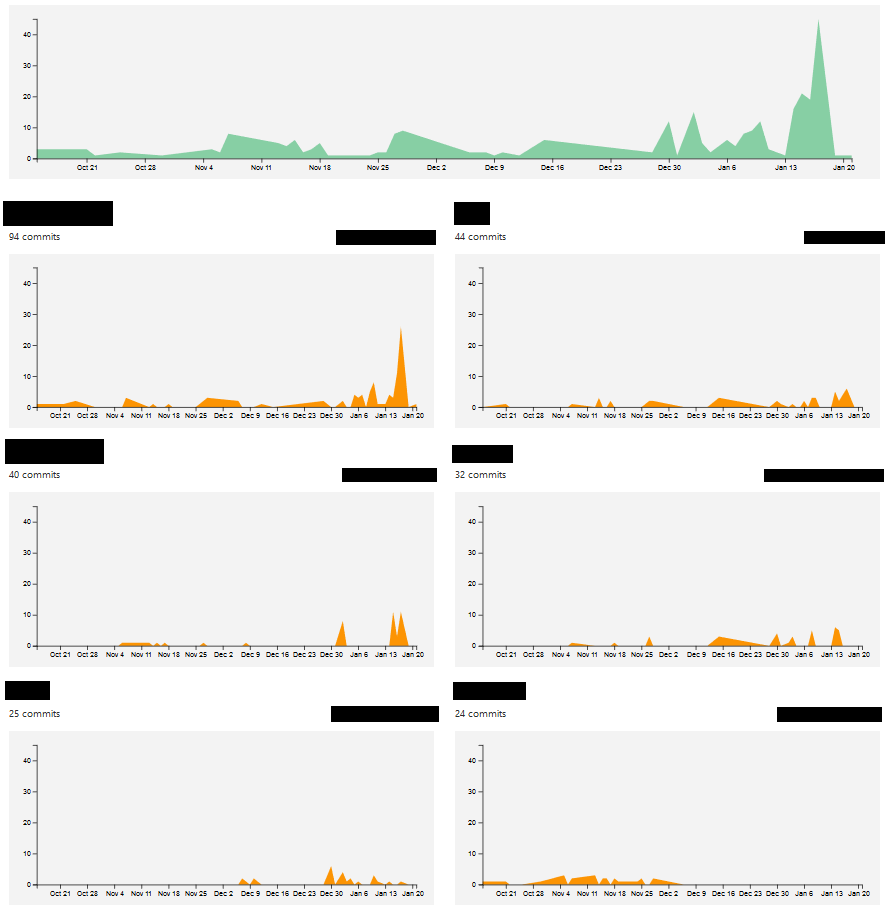
\includegraphics[scale=0.4]{slike/aktivnost.PNG} %veličina slike u odnosu na originalnu datoteku i pozicija slike
			\centering
			\caption{Primjer slike s potpisom}
			\label{fig:promjene}
		\end{figure}
		
		\begin{figure}[H]
			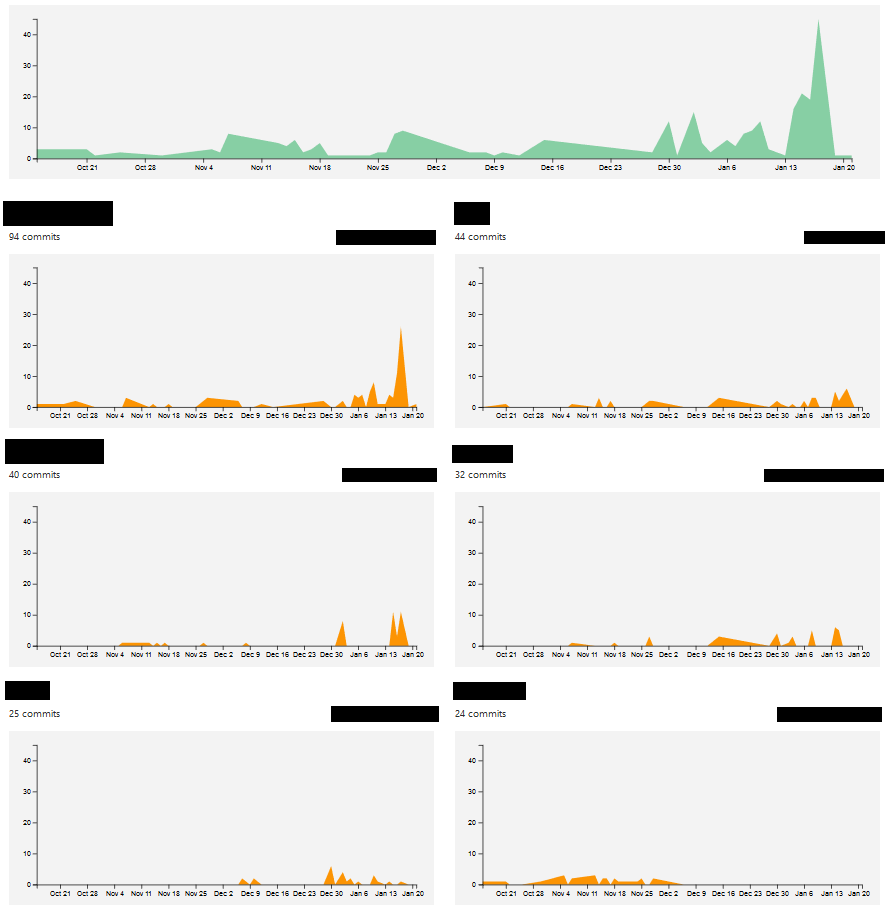
\includegraphics[width=\textwidth]{slike/aktivnost.PNG} %veličina u odnosu na širinu linije
			\caption{Primjer slike s potpisom 2}
			\label{fig:promjene2} %label mora biti drugaciji za svaku sliku
		\end{figure}
		
		Referenciranje slike \ref{fig:promjene2} u tekstu.
		
		\eject
		
	
	\chapter{Specifikacija programske potpore}
		
	\section{Funkcionalni zahtjevi}

			
			\noindent \textbf{Dionici:}
			
			\begin{packed_enum}
				
				\item Administrator
				\item Organizator				
				\item Baza podataka
				\item PayPal
				\item Banka
				\item Korisnik
				\item Posjetitelj
				
			\end{packed_enum}
			
			\noindent \textbf{Aktori i njihovi funkcionalni zahtjevi:}
			
			
			\begin{packed_enum}
				\item  \underbar{Administrator (inicijator) može:}
				
				\begin{packed_enum}
					
					\item prijaviti se i odjaviti sa stranice
					\item pregledavati događaje
					\begin{packed_enum}
	
							\item  filtrirati događaje po vremenskom razdoblju
	
					\end{packed_enum}
					\item  upravljanti korisnicima
					\begin{packed_enum}
						
							\item  urediti ili izbrisati korisničke profile
							\item  urediti ili izbrisati objave korisnika
																			
				    \end{packed_enum}
					\item  postavljati cijene članstva
					
				\end{packed_enum}
			
			    \item  \underbar{Organizator (inicijator) može:}
				
				\begin{packed_enum}
					
					\item postaviti događaj
					\begin{packed_enum}
						
						\item  urediti ili izbrisati događaj
						\item  postaviti događaj sa plaćanjem ulaznice i platiti članraninu (Paypalom ili bankovnom karticom)
						
					\end{packed_enum}
					\item prijaviti se i odjaviti sa stranice
					\item napravi profil
					\item prikazati profil i urediti ga
					\item pregledavati događaje
					\begin{packed_enum}
	
						\item filtriraj događaje po vremenskom razdoblju
	
					\end{packed_enum}
					
				\end{packed_enum}
				
				\item  \underbar{Baza podataka (sudionik):}	
							
				\begin{packed_enum}				
				
					\item pohranjuje zapise o korisnicima i događajima
					\item pohranjuje iskazane interese za događaje
					\item pohranjuje recenzije događaja			
					\item pohranjuje informacije o cijenama članstva
					\item omogućuje prijavu i odjavu sa stranice (token)
				\end{packed_enum}

				\item  \underbar{PayPal (sudionik):}

				\begin{packed_enum}

				\item Odobrava transakcije potrebne za platiti članarinu

				\end{packed_enum}				
				
				\item  \underbar{Banka (sudionik):}				
				
				\begin{packed_enum}
						
				\item Odobrava transakcije potrebne za platiti članarinu 					
					
				\end{packed_enum}
			    
			    \item  \underbar{Korisnik  (inicijator) može:}
				
				\begin{packed_enum}
					
					\item prijaviti se i odjaviti sa stranice
					\item napravi profil
					\item prikazati profil i urediti ga
					\item pregledavati događaje
					\begin{packed_enum}
	
					\item  filtrirati događaje po vremenskom razdoblju
	
					\end{packed_enum}
					
				\end{packed_enum}
					
				\item  \underbar{Posjetitelj   (inicijator) može:}
					
					\begin{packed_enum}
					\item iskazati interese za događaj („sigurno dolazim“, „možda dolazim“, „ne dolazim“)
					\item recenzirati događaj	
					\item prijaviti se i odjaviti sa stranice
					\item napraviti profil
					\item prikazati profil i urediti ga
					\item uključiti obavijesti o najnovijim događajima po kriterijima: vrsta događanja i područje
					\item pregledavati događaje
					\begin{packed_enum}
	
						\item  filtrirati događaje po vremenskom razdoblju
	
					\end{packed_enum}
															
					\end{packed_enum}
												
			\end{packed_enum}
			
			\eject 
			
			
				
			\subsection{Obrasci uporabe}
				
				\textbf{\textit{dio 1. revizije}}
				
				\subsubsection{Opis obrazaca uporabe}
					\textit{Funkcionalne zahtjeve razraditi u obliku obrazaca uporabe. Svaki obrazac je potrebno razraditi prema donjem predlošku. Ukoliko u nekom koraku može doći do odstupanja, potrebno je to odstupanje opisati i po mogućnosti ponuditi rješenje kojim bi se tijek obrasca vratio na osnovni tijek.}\\
					

					\noindent \underbar{\textbf{UC$<$broj obrasca$>$ -$<$ime obrasca$>$}}
					\begin{packed_item}
	
						\item \textbf{Glavni sudionik: }$<$sudionik$>$
						\item  \textbf{Cilj:} $<$cilj$>$
						\item  \textbf{Sudionici:} $<$sudionici$>$
						\item  \textbf{Preduvjet:} $<$preduvjet$>$
						\item  \textbf{Opis osnovnog tijeka:}
						
						\item[] \begin{packed_enum}
	
							\item $<$opis korak jedan$>$
							\item $<$opis korak dva$>$
							\item $<$opis korak tri$>$
							\item $<$opis korak četiri$>$
							\item $<$opis korak pet$>$
						\end{packed_enum}
						
						\item  \textbf{Opis mogućih odstupanja:}
						
						\item[] \begin{packed_item}
	
							\item[2.a] $<$opis mogućeg scenarija odstupanja u koraku 2$>$
							\item[] \begin{packed_enum}
								
								\item $<$opis rješenja mogućeg scenarija korak 1$>$
								\item $<$opis rješenja mogućeg scenarija korak 2$>$
								
							\end{packed_enum}
							\item[2.b] $<$opis mogućeg scenarija odstupanja u koraku 2$>$
							\item[3.a] $<$opis mogućeg scenarija odstupanja  u koraku 3$>$
							
						\end{packed_item}
					\end{packed_item}
				
					
				\subsubsection{Dijagrami obrazaca uporabe}
					
					\textit{Prikazati odnos aktora i obrazaca uporabe odgovarajućim UML dijagramom. Nije nužno nacrtati sve na jednom dijagramu. Modelirati po razinama apstrakcije i skupovima srodnih funkcionalnosti.}
				\eject		
				
			\subsection{Sekvencijski dijagrami}
				
				\textbf{\textit{dio 1. revizije}}\\
				
				\textit{Nacrtati sekvencijske dijagrame koji modeliraju najvažnije dijelove sustava (max. 4 dijagrama). Ukoliko postoji nedoumica oko odabira, razjasniti s asistentom. Uz svaki dijagram napisati detaljni opis dijagrama.}
				\eject
	
		\section{Ostali zahtjevi}
		
			\textbf{\textit{dio 1. revizije}}\\
		 
			 \textit{Nefunkcionalni zahtjevi i zahtjevi domene primjene dopunjuju funkcionalne zahtjeve. Oni opisuju \textbf{kako se sustav treba ponašati} i koja \textbf{ograničenja} treba poštivati (performanse, korisničko iskustvo, pouzdanost, standardi kvalitete, sigurnost...). Primjeri takvih zahtjeva u Vašem projektu mogu biti: podržani jezici korisničkog sučelja, vrijeme odziva, najveći mogući podržani broj korisnika, podržane web/mobilne platforme, razina zaštite (protokoli komunikacije, kriptiranje...)... Svaki takav zahtjev potrebno je navesti u jednoj ili dvije rečenice.}
			 
			 
			 
	
	\chapter{Arhitektura i dizajn sustava}
		
	Arhitektura našeg sustava temeljit će se na kombinaciji modernih tehnologija kako bismo ostvarili funkcionalan i skalabilan sustav. Sustav će se podijeliti na tri ključna podsustava: 
	\begin{itemize}
		\item 	\textit{\textbf{Web poslužitelj}}		
		\item 	\textit{\textbf{Web klijent}}	
		\item 	\textit{\textbf{Baza podataka}}
	\end{itemize}
	
	\begin{figure}[H]
		
\includegraphics[scale=0.75]{slike/skica arh.png} %veličina slike u odnosu na originalnu datoteku i pozicija slike
		\centering
		\caption{Arhitektura sustava}
		\label{fig:promjene}
	\end{figure}
	
	Organizacija će biti usklađena s MVC (Model-View-Controller) konceptom, što će omogućiti neovisnost između različitih dijelova sustava te olakšati razvoj, ispitivanje i dodavanje novih funkcionalnosti.
	
	\textit{\textbf{Web preglednik}}, kao program koji omogućuje korisnicima pregled web-stranica i multimedijalnih sadržaja, igra ključnu ulogu kao sučelje između web klijenta i web aplikacije. Klijenti, putem web preglednika, šalju zahtjeve web poslužitelju kako bi pristupili željenim resursima.
	
	\textit{\textbf{Web poslužitelj}} je osnova rada web aplikacije i odgovoran je za komunikaciju između klijenta i aplikacije. Komunikacija se odvija putem HTTP protokola, koji omogućuje prijenos informacija na webu. Poslužitelj pokreće web aplikaciju i prosljeđuje joj zahtjeve koje prima od klijenata.	

	\textit{\textbf{Web aplikacija}}, smještena na poslužitelju, obrađuje zahtjeve korisnika. Ovisno o tim zahtjevima, pristupa poslužitelju baze podataka i na temelju dobivenih podataka, putem web poslužitelja, šalje odgovor korisnicima. Aplikacija se sastoji od backend i frontend dijela, koji se razvijaju koristeći različite tehnologije u skladu s opisanom arhitekturom sustava. Konkretno, za backend dio koristit ćemo Spring, dok će za frontend biti korišten React, što je u skladu s MVC načelima.
		
	Ključna karakteristika arhitekturnog obrasca MVC-a je nezavisan razvoj pojedinih dijelova aplikacije. Ova karakteristika rezultira jednostavnijim ispitivanjem, kao i olakšanim razvojem i dodavanjem novih svojstava u sustav.
	
	MVC koncept sastoji se od tri osnovna dijela:
	
	\begin{itemize}
		\item 	\textit{\textbf{Model:}}	središnja komponenta sustava koja predstavlja dinamičke strukture podataka neovisne o korisničkom sučelju. Model upravlja podacima, logikom i pravilima aplikacije, primajući ulazne podatke od Controllera
		\item 	\textit{\textbf{View:}}	odgovara za prikaz podataka, poput grafičkih elemenata. Moguć je različiti prikaz istih informacija, kao što su grafički ili tablični prikazi podataka
		\item 	\textit{\textbf{Controller:}} primarno prima ulazne podatke od korisnika i prilagođava ih za daljnju interakciju s Modelom ili Viewom. Kontrolira korisničke zahtjeve i izvodi daljnju interakciju s ostalim elementima sustava
	\end{itemize}
	
	Ovaj pristup omogućuje jasnu organizaciju sustava i olakšava daljnji razvoj i održavanje.

		

				
		\section{Baza podataka}
			
			
		Kao sustav za upravljanje bazama podataka za našu aplikaciju odabrali smo PostgreSQL. To je otvoren sustav za upravljanje bazama koji omogućuje pohranu, upravljanje i analizu podataka.
			
		Sama baza podataka sadržavat će sedam tablica. One će služiti za pohranu podataka o korisnicima te njihovom korištenju aplikacije. Korištenje će se spremati u obliku događaja koje stvaraju ili posjećuju te recenzija koje pišu za određene događaje. Isto tako spremat će se sama zainteresiranost za događaje te notifikacije koje posjetitelji žele primati za događaje s određenim karakteristikama.
			
		Sami odabir PostgreSQL-a je u njegovoj pouzdanosti, skalabilnosti i podrške za napredne SQL funkcionalnosti, što će nam omogućiti lakše te učinkovitije upravljanje podacima.
			Baza podataka ove aplikacije sastoji se od sljedećih entiteta: 
			\begin{itemize}
			\item 	Korisnik
			\item 	Organizator	
			\item 	Događaj
			\item 	Recenzija
			\item 	Zainteresiranost
			\item 	Notifikacija
			\item 	Misc
		\end{itemize}
		
		
			\subsection{Opis tablica}
			

				\textbf{Korisnik} -  ovaj entitet sadržava sve važne informacije o korisniku aplikacije. Sadrži atribute: korisnikId koji je automatski dodijeljen, username, password, email i uloga u aplikaciji. Ovaj entitet u vezi je Many-to-One s entitetom organizator preko atributa organizatorId.
				
				
				\begin{longtblr}[
					label=none,
					entry=none
					]{
						width = \textwidth,
						colspec={|X[7,l]|X[6, l]|X[20, l]|}, 
						rowhead = 1,
					} %definicija širine tablice, širine stupaca, poravnanje i broja redaka naslova tablice
					\hline \SetCell[c=3]{c}{\textbf{korisnik}}	 \\ \hline[3pt]
					\SetCell{LightGreen}korisnikId & INT	&  	Primarni ključ tablice, dodjeljuje se automatski  	\\ \hline
					username	& VARCHAR & Jedinstveno ime koje korisnik odabire tijekom registracije  	\\ \hline 
					password & VARCHAR & Lozinka koju korisnik odabire tijekom registracije  \\ \hline 
					email & VARCHAR	&  Jedinstveni email korisnika		\\ \hline 
					uloga & SMALL INT/INT &  Uloga koju korisnik ima unutar aplikacije(admin, posjetitelj, organizator)		\\ \hline 
				\end{longtblr}
				
							\textbf{Organizator } -  Ovaj entitet sadržava informacije o organizatoru događaja. Sadrži atribute: organizatorId, nazivOrganizacije, adresa, poveznica, clanarina. Ovaj entitet u vezi je One-to-Many s entitetom dogadaj preko atributa organizatorId.
			
			
			\begin{longtblr}[
				label=none,
				entry=none
				]{
					width = \textwidth,
					colspec={|X[9,l]|X[6, l]|X[20, l]|}, 
					rowhead = 1,
				} %definicija širine tablice, širine stupaca, poravnanje i broja redaka naslova tablice
				\hline \SetCell[c=3]{c}{\textbf{organizator}}	 \\ \hline[3pt]
				\SetCell{LightGreen}organizatorId & INT	&  	Primarni ključ tablice, ujedno i strani ključ iz tablice korisnik 	\\ \hline
				nazivOrganizacije	& VARCHAR & Naziv organizacije kojoj pripada organizator  	\\ \hline 
				adresa & VARCHAR & Adresa organizacije  \\ \hline 
				poveznica & VARCHAR	&  Poveznica na web stranicu organizacije		\\ \hline 
				clanarina & BOOLEAN &  Plaćena članarina		\\ \hline 
			\end{longtblr}
			
							\textbf{Događaj} -  ovaj entitet sadržava informacije o događaju. Sadrži atribute: dogadajId, organizatorId, nazivDogadaja, vrsta, lokacija, trajanje, vrijemePocetka, cijenaUlaznice, opis, galerija. Ovaj entitet u vezi je Many-to-One s entitetom Organizator preko atributa organizatorId te u vezi One-to-Many s entitetom recenzija preko atributa dogadajId.
			
			
			\begin{longtblr}[
				label=none,
				entry=none
				]{
					width = \textwidth,
					colspec={|X[7,l]|X[6, l]|X[20, l]|}, 
					rowhead = 1,
				} %definicija širine tablice, širine stupaca, poravnanje i broja redaka naslova tablice
				\hline \SetCell[c=3]{c}{\textbf{dogadaj}}	 \\ \hline[3pt]
				\SetCell{LightGreen}dogadajId & INT	&  	Primarni ključ tablice, dodjeljuje se automatski  	\\ \hline			
				\SetCell{LightBlue} organizatorId	& INT & Strani ključ iz tablice organizator koji se odnosi na njegov ID  	\\ \hline 
				nazivDogadaja	& VARCHAR & Naziv događaja  	\\ \hline 
				vrsta & VARCHAR & Vrsta događaja(koncert, kazališna predstava ...)  \\ \hline 
				lokacija & VARCHAR	&  Lokacija događaja		\\ \hline 
				opisLokacije & VARCHAR & Kratki opis lokacije, adresa, kat …	\\ \hline 
				trajanje & INTERVAL & Trajanje događaja u danima \\ \hline 
				vrijemePocetka & TIMESTAMP & Datum i vrijeme početka događaja \\ \hline 
				cijenaUlaznice & NUMERIC & Cijena ulaznice na događaj \\ \hline 
				opis & VARCHAR & Kratki opis samog događaja \\ \hline 
				galerija & VARCHAR & Link do web stranice gdje se nalaze video snimke ili fotografije \\ \hline  
			\end{longtblr}
			
							\textbf{Recenzija} -  ovaj entitet sadržava informacije o recenziji događaja. Sadrži atribute: recenzijaId, korisnikId, dogadajId, tekst, ocjena. Ovaj entitet u vezi je Many-to-One s entitetom korisnik preko atributa korisnikId te u vezi Many-to-One s entitetom događaj preko atributa dogadajId.
			
			
			\begin{longtblr}[
				label=none,
				entry=none
				]{
					width = \textwidth,
					colspec={|X[7,l]|X[6, l]|X[20, l]|}, 
					rowhead = 1,
				} %definicija širine tablice, širine stupaca, poravnanje i broja redaka naslova tablice
				\hline \SetCell[c=3]{c}{\textbf{recenzija}}	 \\ \hline[3pt]
				\SetCell{LightGreen}recenzijaId & INT	&  	Primarni ključ tablice, dodjeljuje se automatski  	\\ \hline
				\SetCell{LightBlue}korisnikId	& INT & Strani ključ iz tablice korisnik koji se odnosi na njegov ID	\\ \hline 
				\SetCell{LightBlue}dogadajId & INT & Strani ključ iz tablice dogadaj koji se odnosi na njegov ID \\ \hline 
				tekst & VARCHAR	&  Kratki tekst recenzije	\\ \hline 
				ocjena & SMALL INT/INT & Ocjena od 1-5, opcionalna	\\ \hline 
			\end{longtblr}
			
							\textbf{Zainteresiranost} -  ovaj entitet sadržava informacije o zainteresiranosti posjetitelja za određeni događaj. Sadrži atribute: zainteresiranostId, posjetiteljId, dogadajId, kategorija. Ovaj entitet u vezi je Many-to-One s entitetom korisnik preko atributa posjetiteljId te u vezi Many-to-One s entitetom dogadaj preko atributa dogadajId.
			
			
			\begin{longtblr}[
				label=none,
				entry=none
				]{
					width = \textwidth,
					colspec={|X[9,l]|X[6, l]|X[20, l]|}, 
					rowhead = 1,
				} %definicija širine tablice, širine stupaca, poravnanje i broja redaka naslova tablice
								\hline \SetCell[c=3]{c}{\textbf{zainteresiranost}}	 \\ \hline[3pt]
				\SetCell{LightGreen}zainteresiranostId & INT	&  	Primarni ključ tablice, dodjeljuje se automatski  	\\ \hline
				\SetCell{LightBlue}posjetiteljId	& INT & Strani ključ iz tablice korisnik koji se odnosi na njegov ID	\\ \hline 
				\SetCell{LightBlue}dogadajId & INT & Strani ključ iz tablice dogadaj koji se odnosi na njegov ID \\ \hline 
				kategorija & SMALL INT/INT	&  Jedna od tri kategorije: Sigurno dolazim, možda dolazim ili ne dolazim	\\ \hline 
				
			\end{longtblr}
			
							\textbf{Notifikacija} -  ovaj entitet sadržava informacije o notifikacijama koje će posjetitelji primati vezano uz tražene događaje filtirane po vrsti ili lokaciji. Sadrži atribute: notifikacijaId, posjetiteljId, vrsta, lokacija. Ovaj entitet u vezi je Many-to-One s entitetom korisnik preko atributa korisnikId te u vezi Many-to-One s entitetom dogadaj preko atributa vrsta i lokacija.
			
			
			\begin{longtblr}[
				label=none,
				entry=none
				]{
					width = \textwidth,
					colspec={|X[7,l]|X[6, l]|X[20, l]|}, 
					rowhead = 1,
				} %definicija širine tablice, širine stupaca, poravnanje i broja redaka naslova tablice
				\hline \SetCell[c=3]{c}{\textbf{notifikacija}}	 \\ \hline[3pt]
				\SetCell{LightGreen}notifikacijaId & INT	&  	Primarni ključ tablice, dodjeljuje se automatski  	\\ \hline
				\SetCell{LightBlue}posjetiteljId	& INT & Strani ključ iz tablice korisnik koji se odnosi na njegov ID \\ \hline
				vrsta & VARCHAR & Vrsta događaja za koji posjetitelj želi primiti obavijest o njegovu stvaranju, opcionalno\\ \hline 
				lokacija & VARCHAR	&  Lokacija događaja za koji posjetitelj želi primiti obavijest o njegovu stvaranju, opcionalno		\\ \hline 
			\end{longtblr}
			
			\textbf{misc} -  skraćeno od "miscellaneous", ovaj entitet služi za spremanje globalnih postavki aplikacija u obliku ključ-vrijednost. Sadrži atribute ime i vrijednost.
			
			
			\begin{longtblr}[
				label=none,
				entry=none
				]{
					width = \textwidth,
					colspec={|X[7,l]|X[6, l]|X[20, l]|}, 
					rowhead = 1,
				} %definicija širine tablice, širine stupaca, poravnanje i broja redaka naslova tablice
				\hline \SetCell[c=3]{c}{\textbf{misc}}	 \\ \hline[3pt]
				\SetCell{LightGreen}ime & VARCHAR	&  	Ime (ključ) svojstva  	\\ \hline
				vrijednost & VARCHAR & Vrijednost svojstva \\ \hline
			\end{longtblr}
			
			
			
							
			
			\subsection{Dijagram baze podataka}

				
					\begin{figure}[H]
					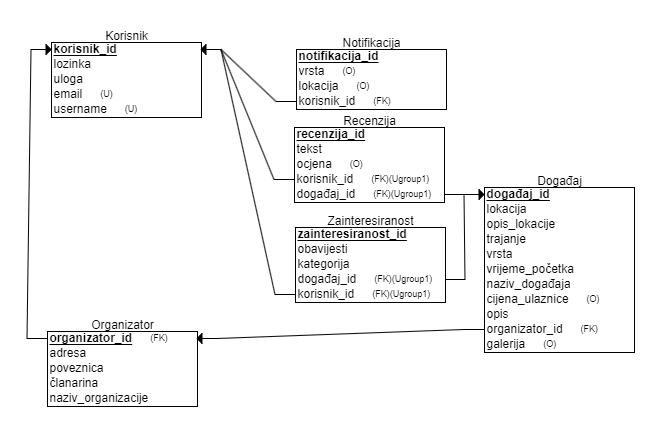
\includegraphics[scale=0.9]{slike/baza.png} %veličina slike u odnosu na originalnu datoteku i pozicija slike
					\centering
					\caption{Dijagram baze podataka}
					\label{fig:promjene}
				\end{figure}
				\eject	
				
			
			
		\section{Dijagram razreda}
		
			Na slikama \textbf{4.3, 4.4, 4.5 i 4.6} su prikazani razredi koji pripadaju \textit{backend} dijelu projekta te oni predstavljaju i odgovaraju stvarnom stanju implementacije sustava te su generirani iz same implementacije. 
			\newline
			\newline
			Razredi prikazani na slici \textbf{4.3} su razredi kontroleri. Ti razredi su ključni dijelovi koji upravljaju pristiglim zahtjevima, određuju rute te obrađuju logiku aplikacije. Obično se koriste za implementaciju HTTP metoda poput \textbf{GET, POST, PUT i DELETE} za obrađivanje zahtjeva koji dolaze od klijenata. Razredi koji imaju svoje kontrolere su \textbf{Korisnik, Organizator,  Događaj, Notifikacija i Transakcije}. Na primjeru KorisnikControllera ćemo detaljnije opisati metode i članske varijable koje su korištene za spajanje sa servisnim slojem.
			\newline
			
			\textbf{KorisnikController} ima metode: 
			\begin{itemize}
				\item getAll - vraća listu Korisnika
				\item delete - kao argument prima ID Korisnika te ga briše ukoliko postoji
				\item validate - prima Korisnika te vraća ResponseEntity, služi validaciji Korisnika
				\item register - kao argument prima KorsnikDTO, a vraća ResponseEntity koji je string
				\item update - služi promjeni i ažuriranju podataka Korisnika
			\end{itemize}
			
			Isto ima i članske varijable tipa KorisnikService i OrganizatorServiceJpa  preko kojih se obavlja poslovna logika (operacije nad podacima, pristupanje bazi podataka ili komunikacija s vanjskim servisima).
			\newline

			Razredi prikazani na slici \textbf{4.4} su razredi servisi. Razredi servisi u Spring Bootu predstavljaju komponente koje sadrže poslovnu logiku aplikacije, pristupaju podacima i obavljaju operacije koje nisu specifične za obradu HTTP zahtjeva. Oni često služe kao posrednici između kontrolera i sloja pristupa podacima (Repository sloj) te obavljaju ključne funkcije za obradu podataka, poslovnu logiku i vanjske integracije. U našem primjeru ostvarili smo prvo sučelja koja smo zatim implementirali.
			Razredi koji imaju svoje servise su \textbf{Korisnik, Organizator, Događaj, Notifikacija, Zainteresiranost, EmailSender, Misc i Recenzija}. Na primjeru KorisnikSerivce ćemo detaljnije opisati metode i članske varijable.
			\newline
			
			\textbf{KorisnikService} sučelje ima metode: 
			\begin{itemize}
				\item listAll - vraća listu Korisnika
				\item findById - prima id kao argument, a ako postoji Korisnik s tim id, njega vraća
				\item findByUsername - prima username kao argument, a ako postoji korisnik s tim usernamom njega vraća
				\item findByEmail - prima email kao argument, a ako postoji korisnik s tim emailom njega vraća
				\item registerUser - kao argument prima KorsnikDTO, a boolean ovisno o uspješnosti
				\item updateUser - kao argument prima KorsnikDTO i ID Korisnika, a boolean ovisno o uspješnosti
				\item deleteUser - kao argument prima Korisnika i briše ga ukoliko postoji
			\end{itemize}
			
			Implementacija sučelja KorisnikService, KorisnikServiceJpa, isto ima i članske varijable tipa KorisnikRepository i PasswordEncoder. Razred repozitorija u Spring Bootu predstavlja sloj pristupa podacima (data access layer) i obično se koristi za komunikaciju s bazom podataka. Ovi repozitoriji pružaju apstrakciju za operacije nad podacima, kao što su dohvaćanje, spremanje, ažuriranje ili brisanje podataka. Instanca PasswordEncoder služi nam za registraciju korisnika te za ažuriranje njegovih podataka kada dolazi do promjene lozinke.
			\newline

			\eject
			Razredi prikazani na slici 4.5. su razredi modeli. Struktura baze podataka u aplikaciji odražava se upravo model razredima; osim što imaju svoje pripadne atributa, razredi također implementiraju metode koje ostvaruju interakciju s bazom podataka. \\ 
			\\ Razred Korisnik reprezentira općeg korisnika aplikacije. Specificira ga atribut "uloga" koja određuje je li korisnik administrator, posjetitelj ili organizator.
			\\ Razred Organizator reprezentira korisnika s organizatorskim računom. Organizatori mogu pregledavati svoje postojeće događaje i postavljati nove događaje.
			\\ Razred Recenzija reprezentira korisnikov osvrt na događaj u obliku ocjene i komentara.
			\\ Razred Notifikacija reprezentira obavijest koja se šalje korisniku. Korisnik ima mogućnost uključiti notifikacije za određenu vrstu događaja te za lokaciju na kojoj se događaji organiziraju.
			\\ Razred Zainteresiranost reprezentira korisnikovu interakciju s postavljenim događajima. Korisnikova zainteresiranost ima tri razine: "sigurno dolazim", "možda dolazim", "ne dolazim".
			\\ Razred Dogadaj reprezentira događaj koji je postavio organizator. Lokacija događaja predstavljena je gradskom četvrti - kvartom.
			\\ Razred Misc skraćeno od ”miscellaneous”, ovaj razred služi za spremanje globalnih postavki aplikacija u obliku ključ-vrijednost. Sadrži atribute ime i vrijednost.
			Osim navedenih razreda na slici su također prikazane enumeracije: 
					Kategorija - kategorija zainteresiranosti korisnika za događaj,
					Kvartovi - kvartovi grada Zagreba gdje se organiziraju događaji,
					Uloga - uloga korisnika i 
					Vrste - različite vrste događaja
			
			\pagebreak
			
			\begin{figure}[H]
				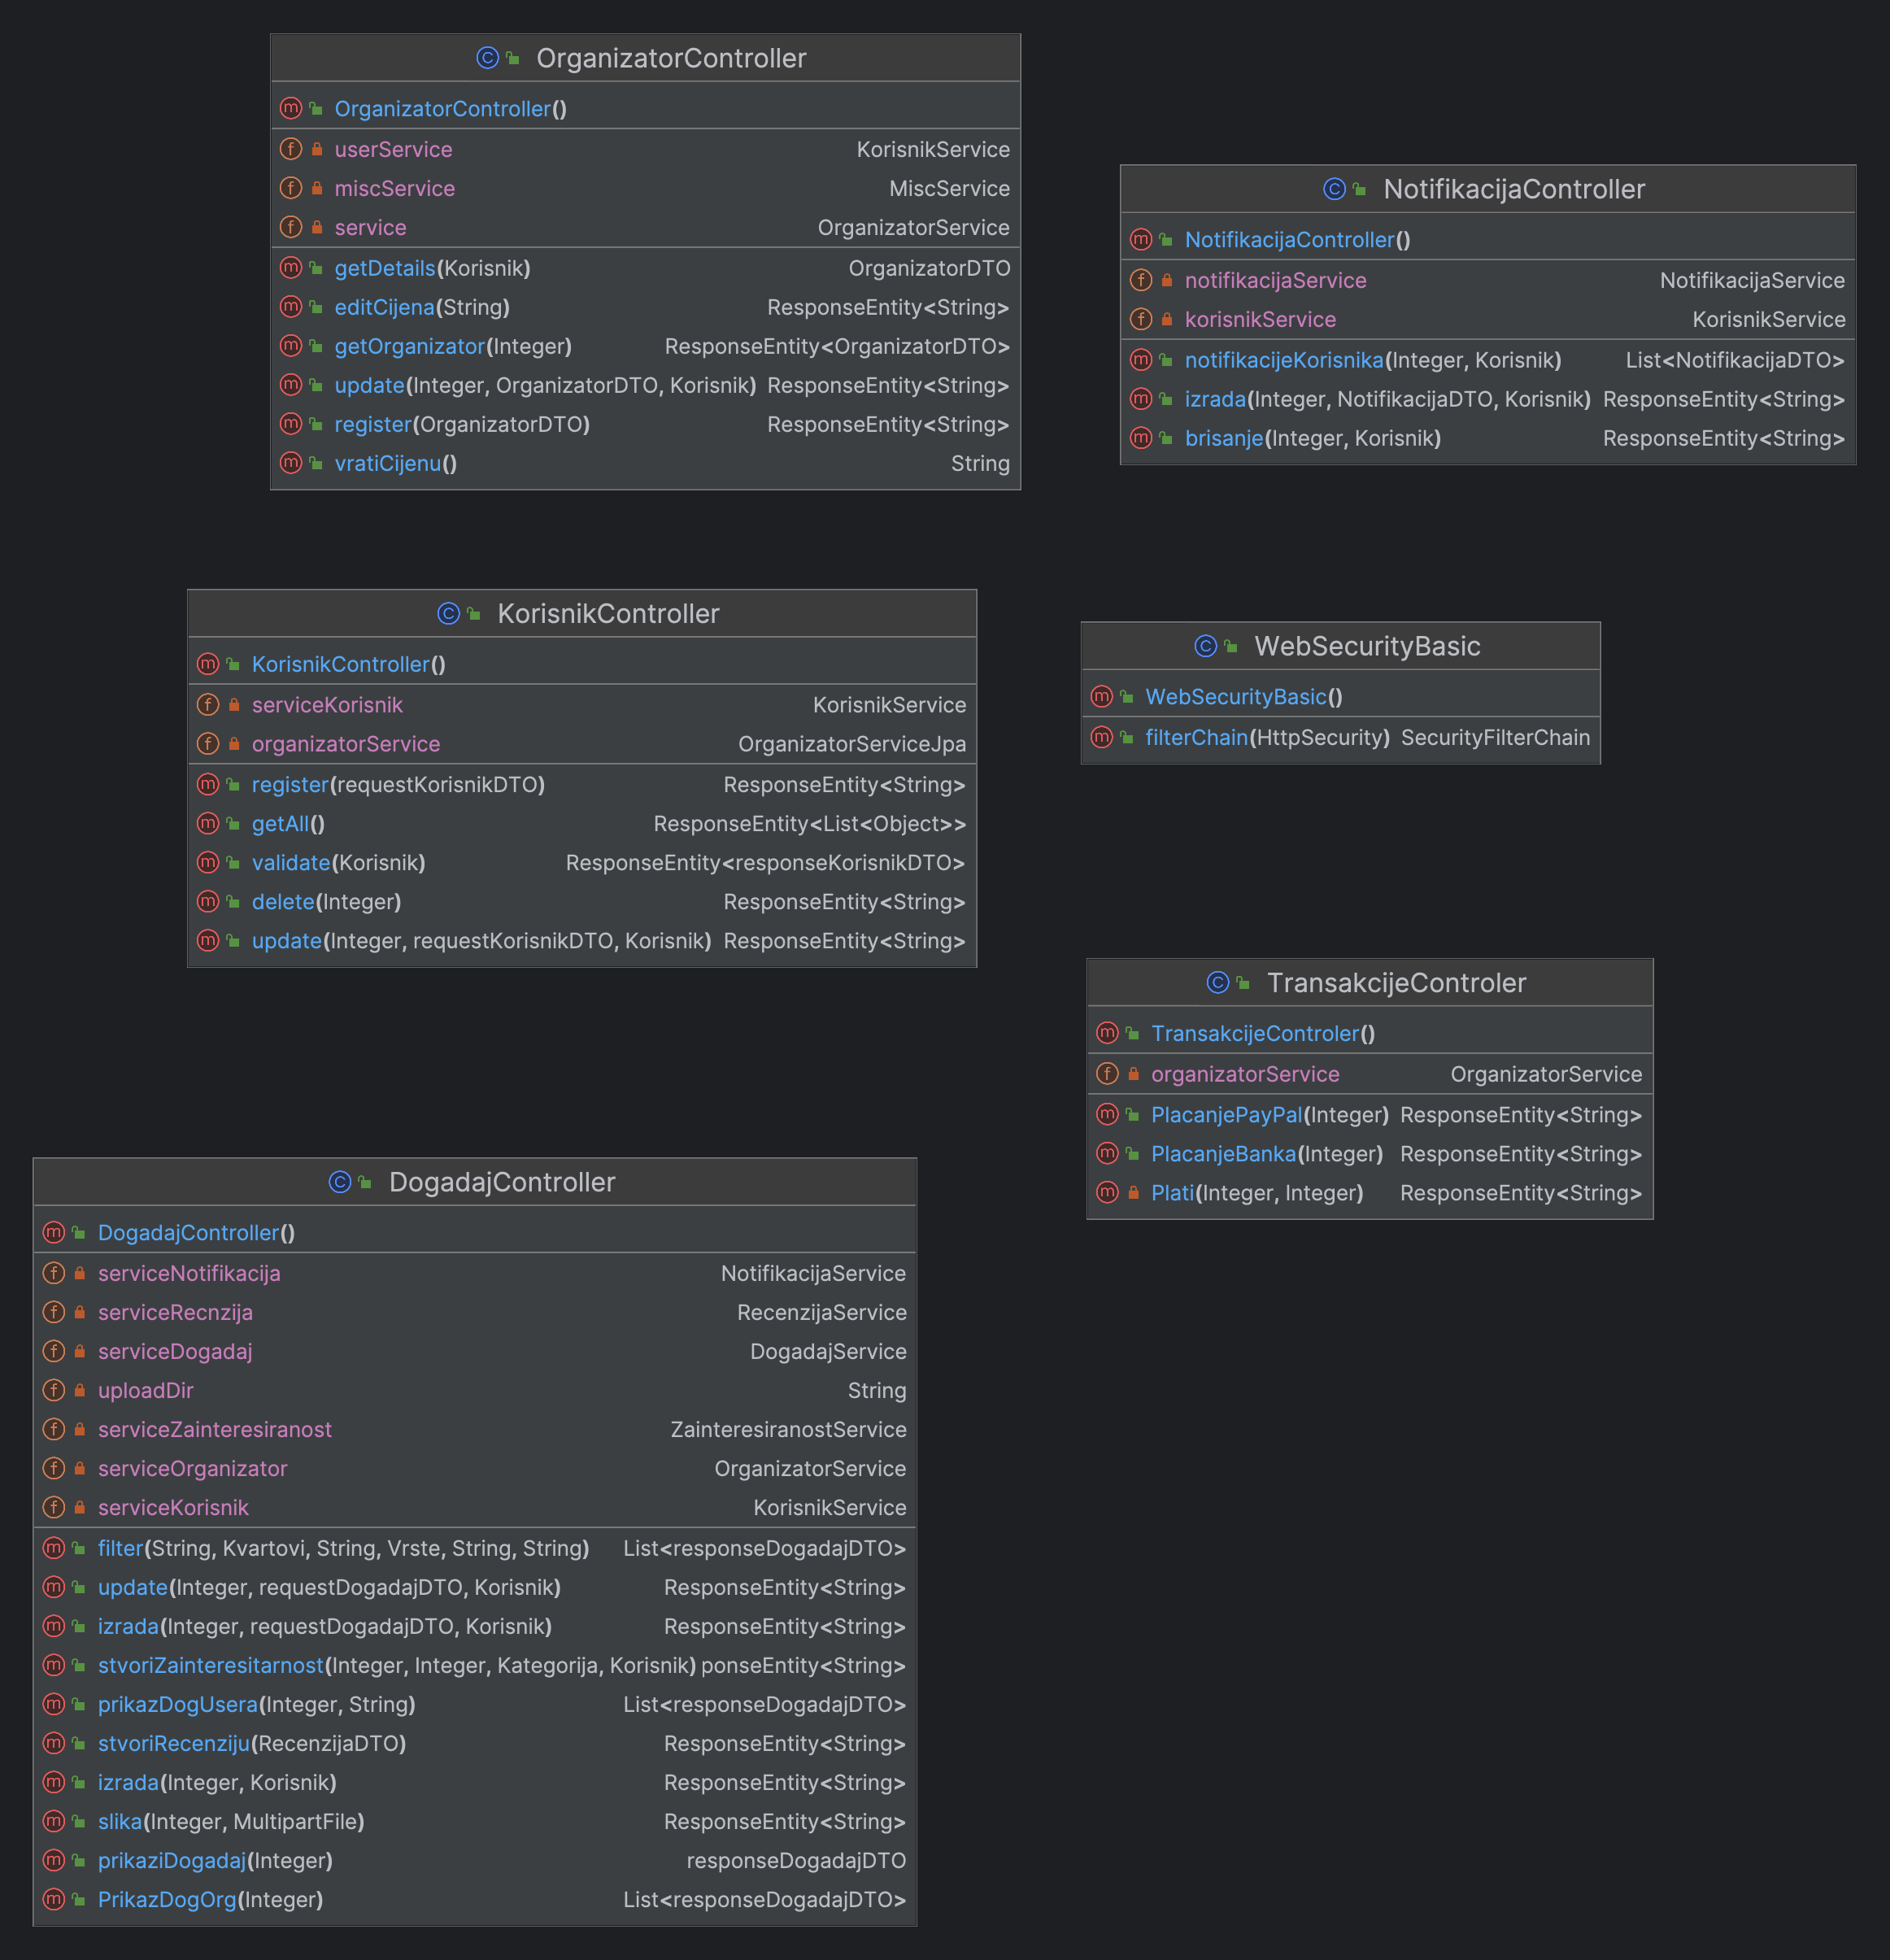
\includegraphics[scale=0.2]{dijagramiKlasa/kontroleri.png} %veličina slike u odnosu na originalnu datoteku i pozicija slike
				\centering
				\caption{Dijagram razreda - Kontroleri}
				\label{fig:promjene}
			\end{figure}
			
			\begin{figure}[H]
				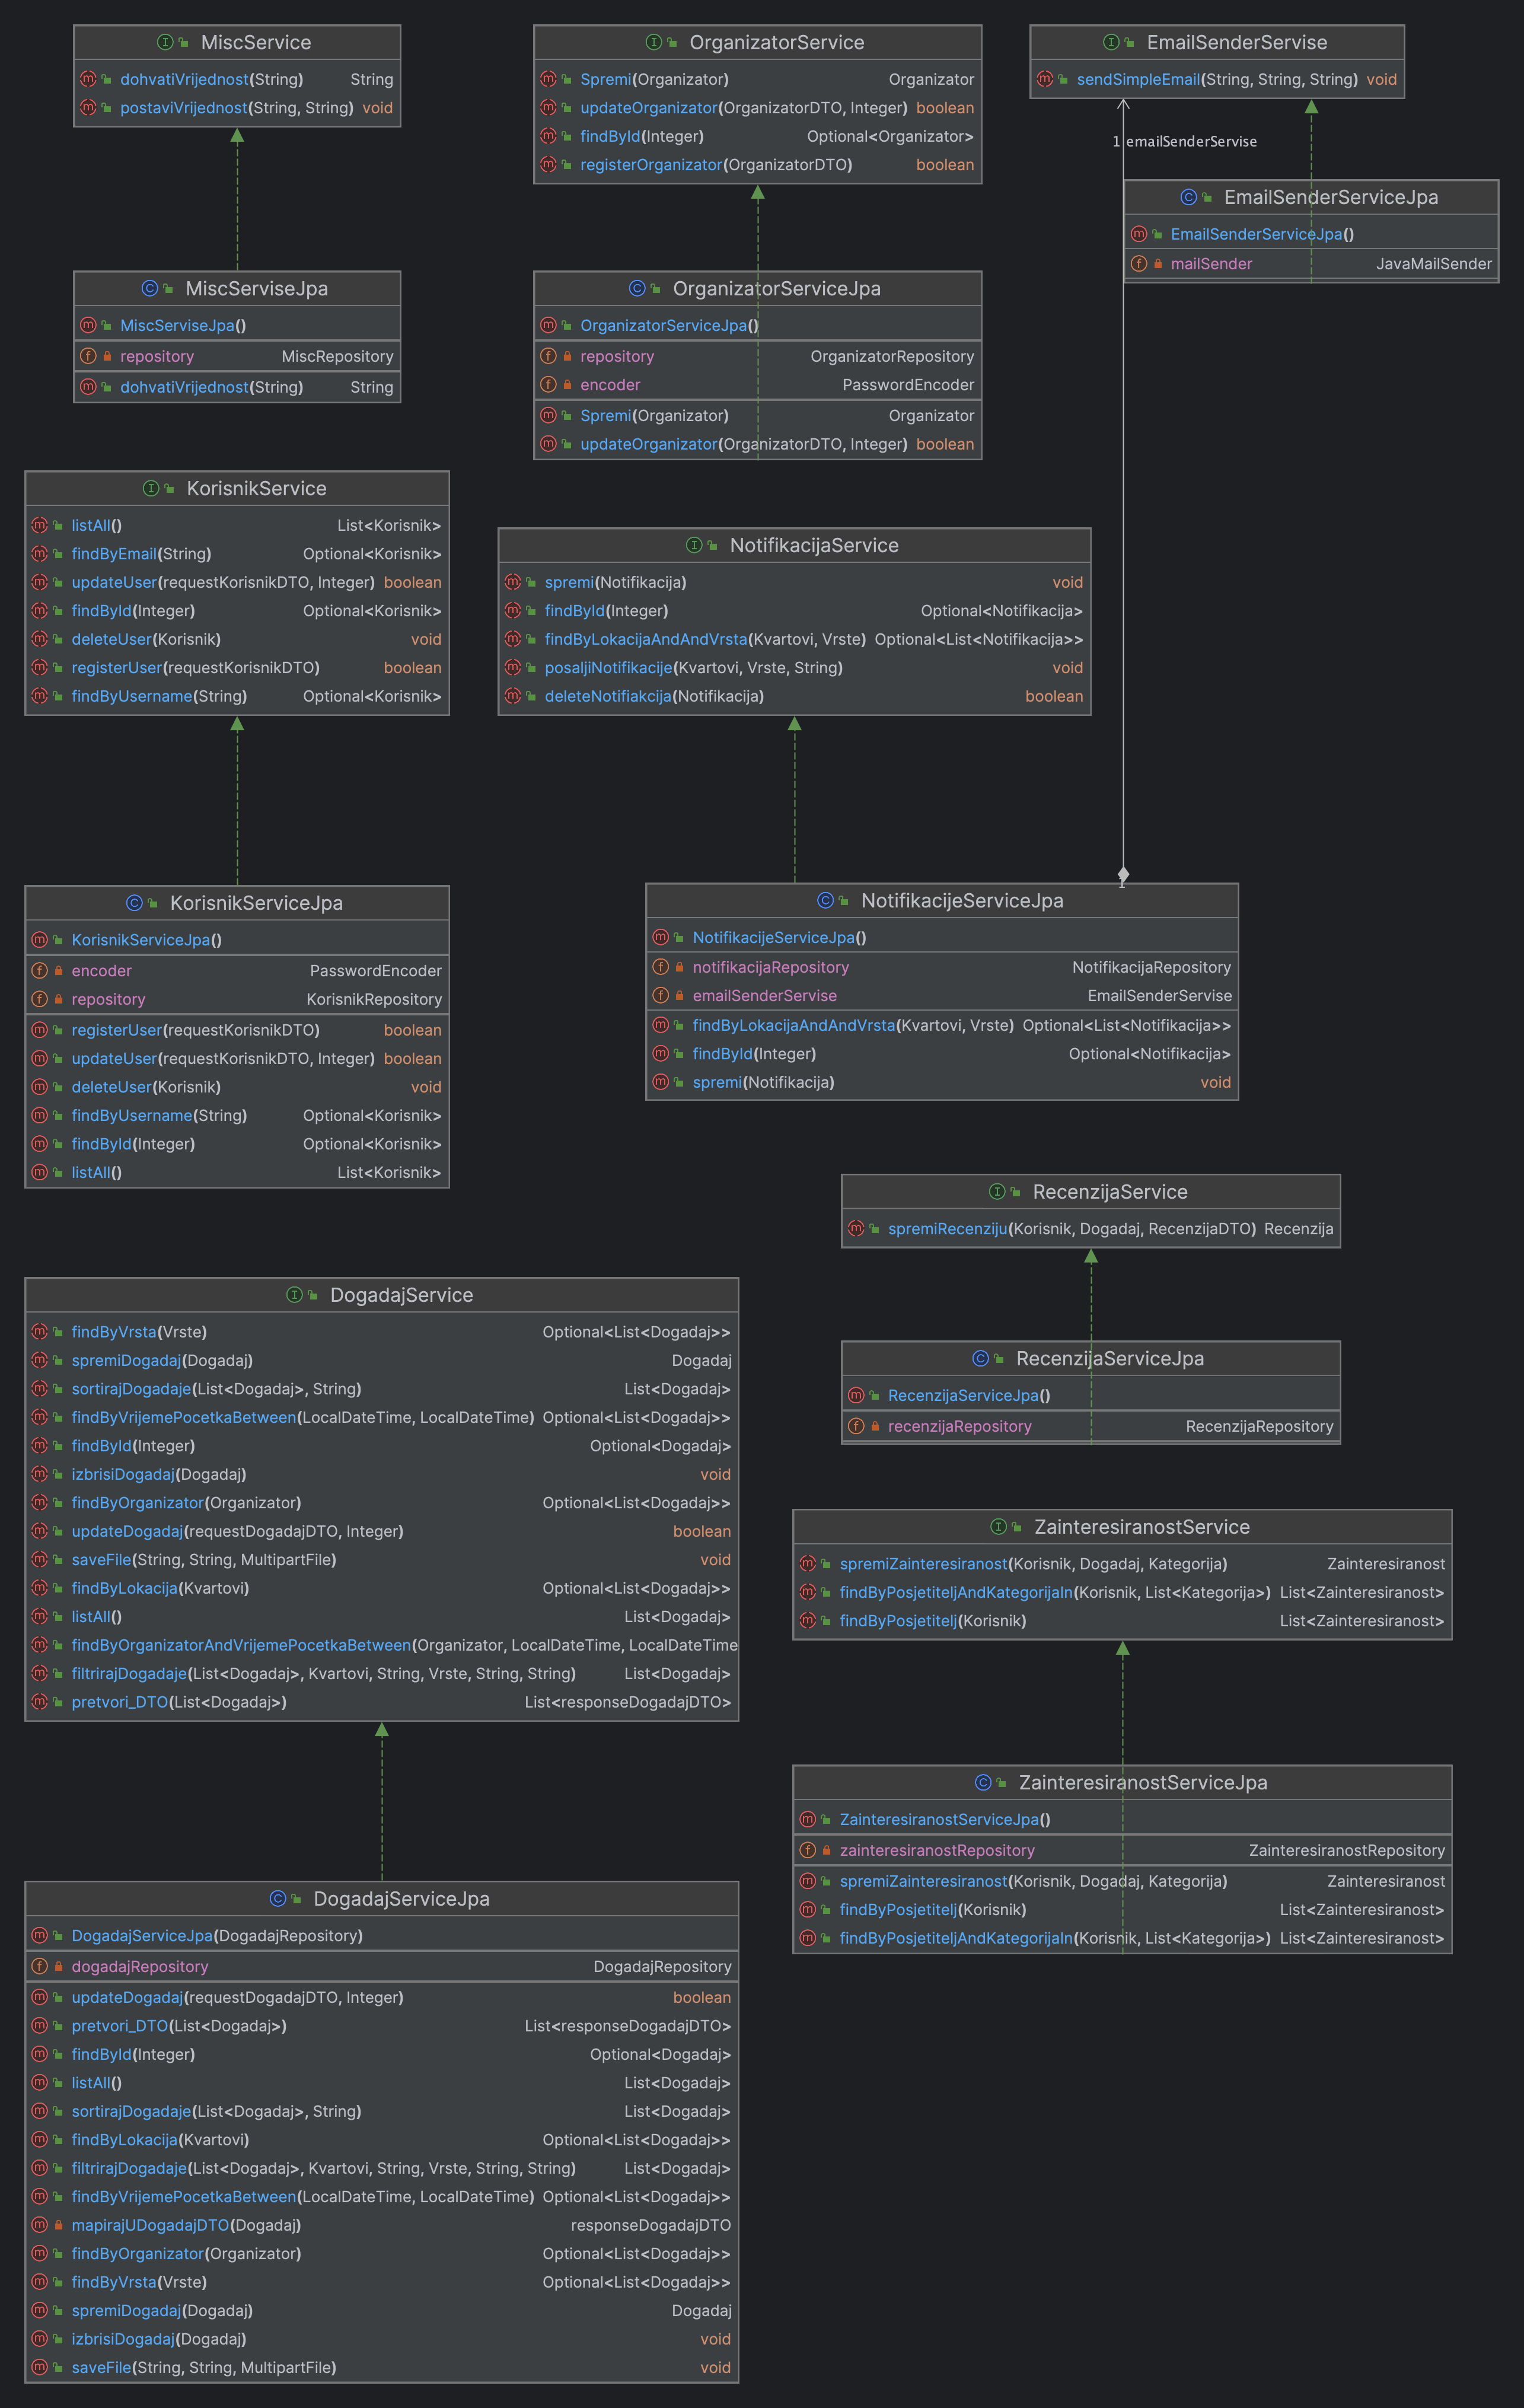
\includegraphics[scale=0.13]{dijagramiKlasa/servisi.png} %veličina slike u odnosu na originalnu datoteku i pozicija slike
				\centering
				\caption{Dijagram razreda - Servisi}
				\label{fig:promjene}
			\end{figure}
			
			\begin{figure}[H]
				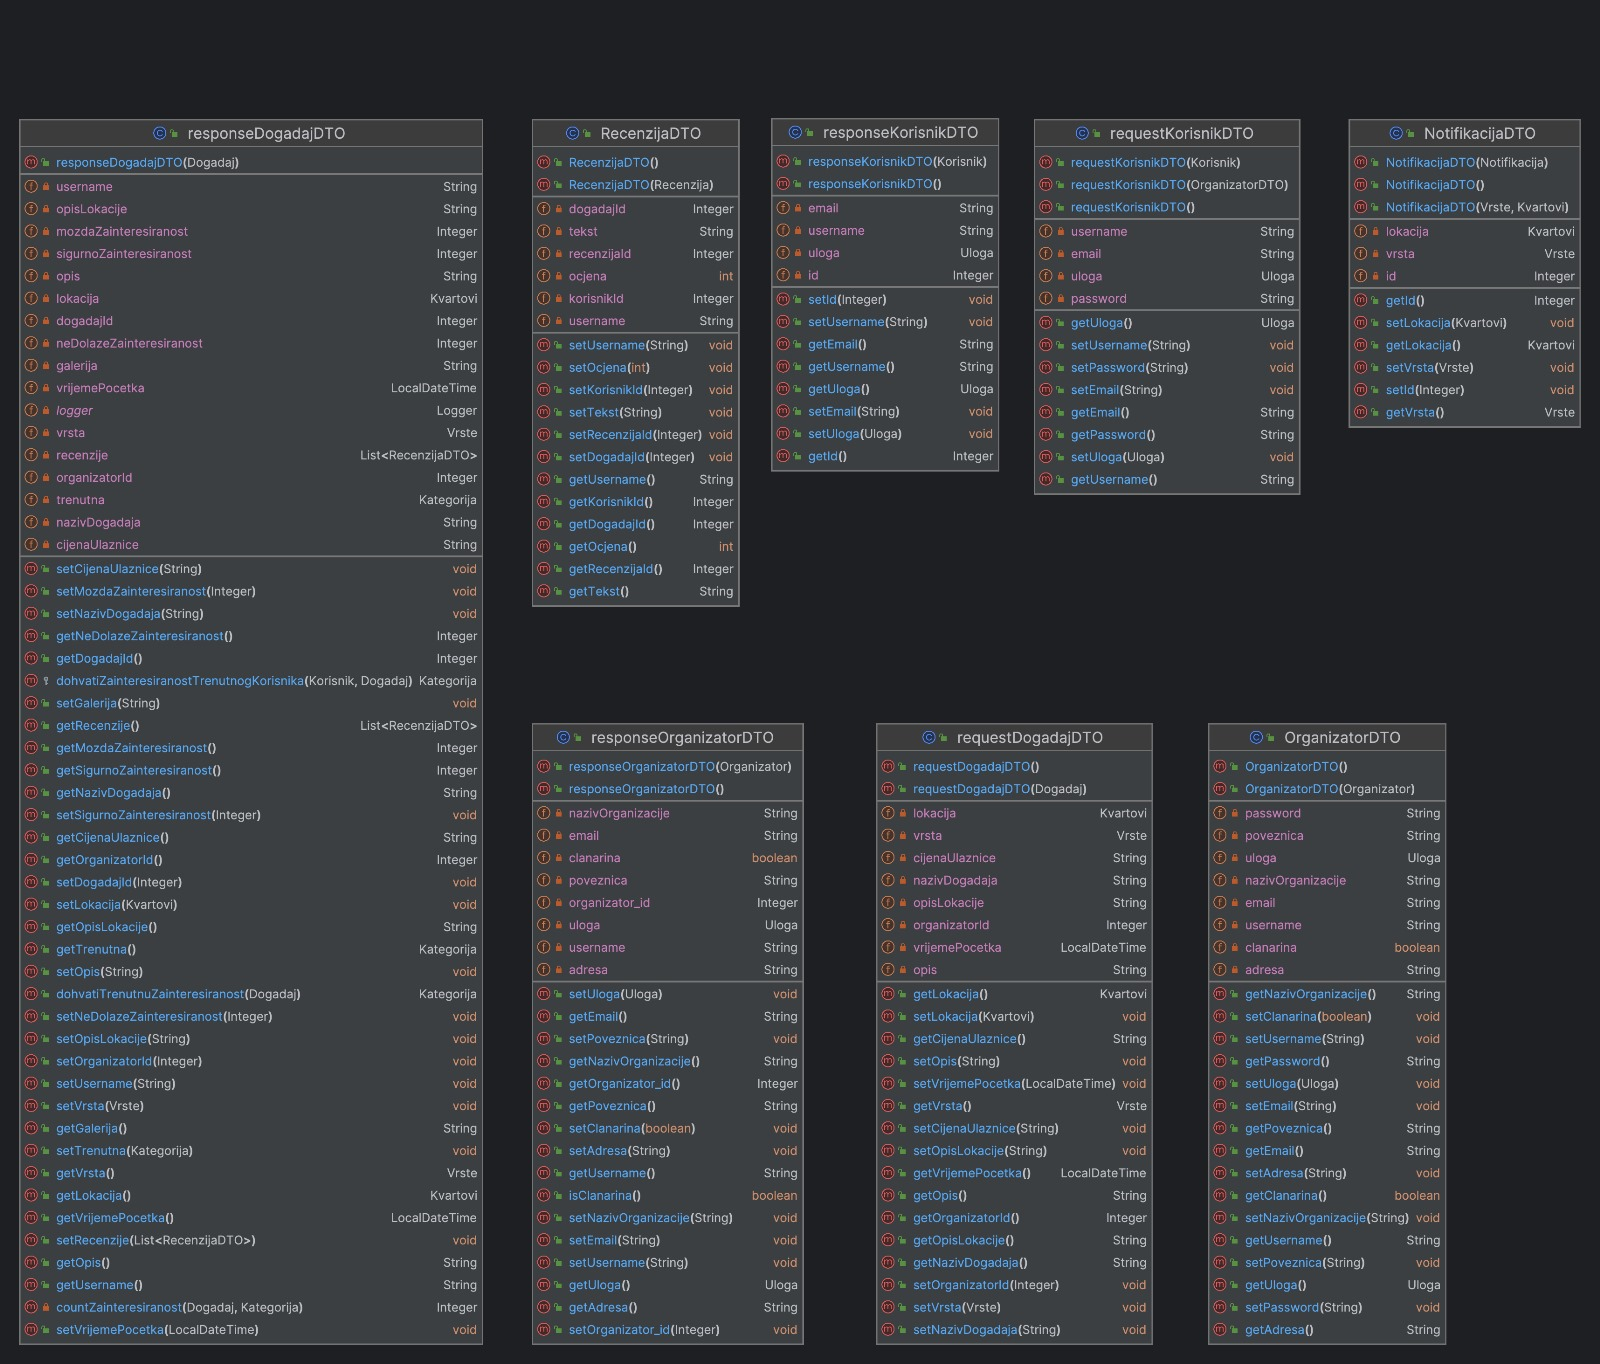
\includegraphics[scale=0.4]{dijagramiKlasa/dijagramRazeda-DTO.jpg} %veličina slike u odnosu na originalnu datoteku i pozicija slike
				\centering
				\caption{Dijagram razreda - Data Transfer Objects}
				\label{fig:promjene}
			\end{figure}
			
			
			\begin{figure}[H]
				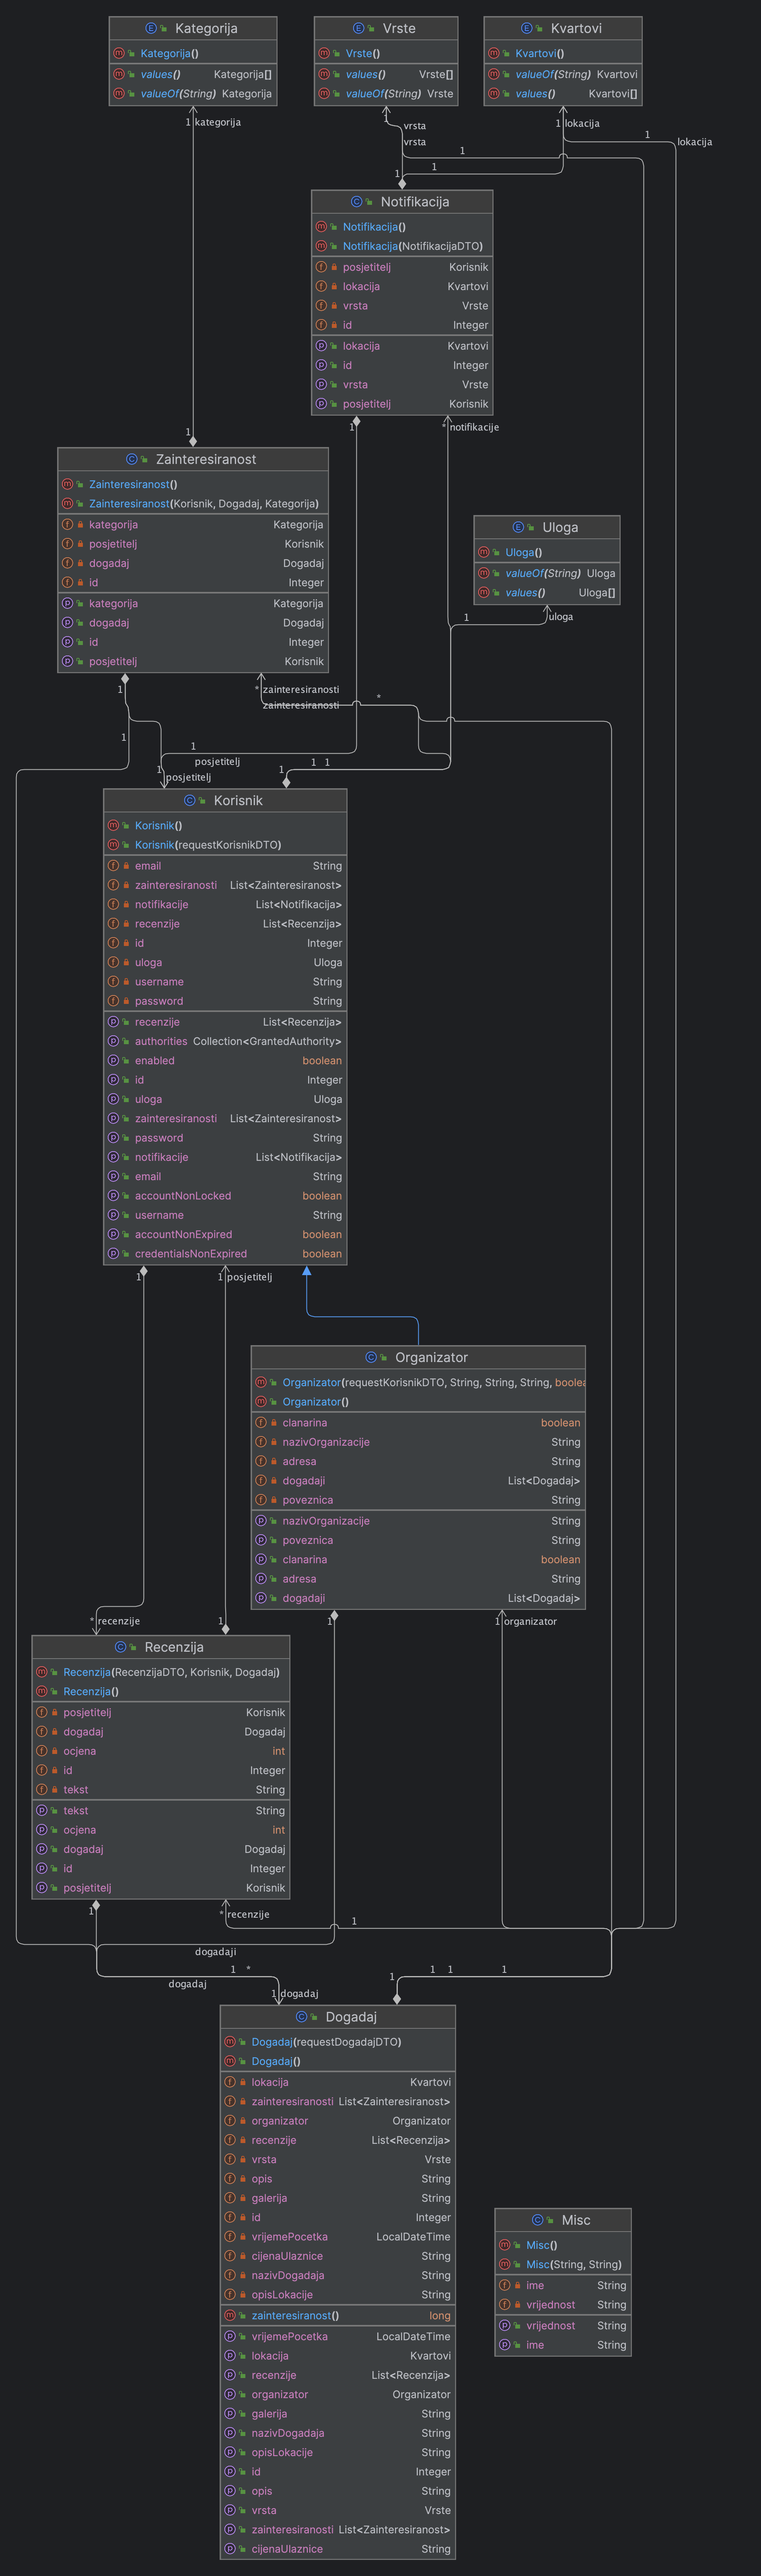
\includegraphics[scale=0.1]{dijagramiKlasa/models.png} %veličina slike u odnosu na originalnu datoteku i pozicija slike
				\centering
				\caption{Dijagram razreda - Models}
				\label{fig:promjene}
			\end{figure}
			
			
			\eject
		
		\section{Dijagram stanja}
			
			
			Dijagram stanja opisuje dinamičko ponašanje dijela sustava u vremenu; prikazuje stanja objekta i prijelaze iz jednog stanja u drugo temeljene na događajima. Na slici 4.7 prikazan je dijagram stanja za korisnika - posjetitelja. Kada se korisnik prijavi prikazuje mu se početna stranica na kojoj su vidljivi događaji, filter pomoću kojeg može odlučiti koje događaje želi pregledati, te navigacijska traka preko kojeg pristupa svim događajima, događajima za koje je označio "Sigurno dolazim" ili "Možda dolazim" te profilu. Klikom na "Moji događaji" prikazuju mu se događaji na koje je prethodno reagirao sa "Sigurno dolazim" ili "Možda dolazim". Ako među ovim događajima postoje događaji koji su završili i nije prošlo 48 sati od njihovog završetka, korisnik za njih može izraditi recenziju. Klikom na korisničko ime - profil prikazuje mu se stranica profila na kojoj može promijeniti osobne podatke te urediti postavke pretplata na obavijesti.
			
			\begin{figure}[H]
			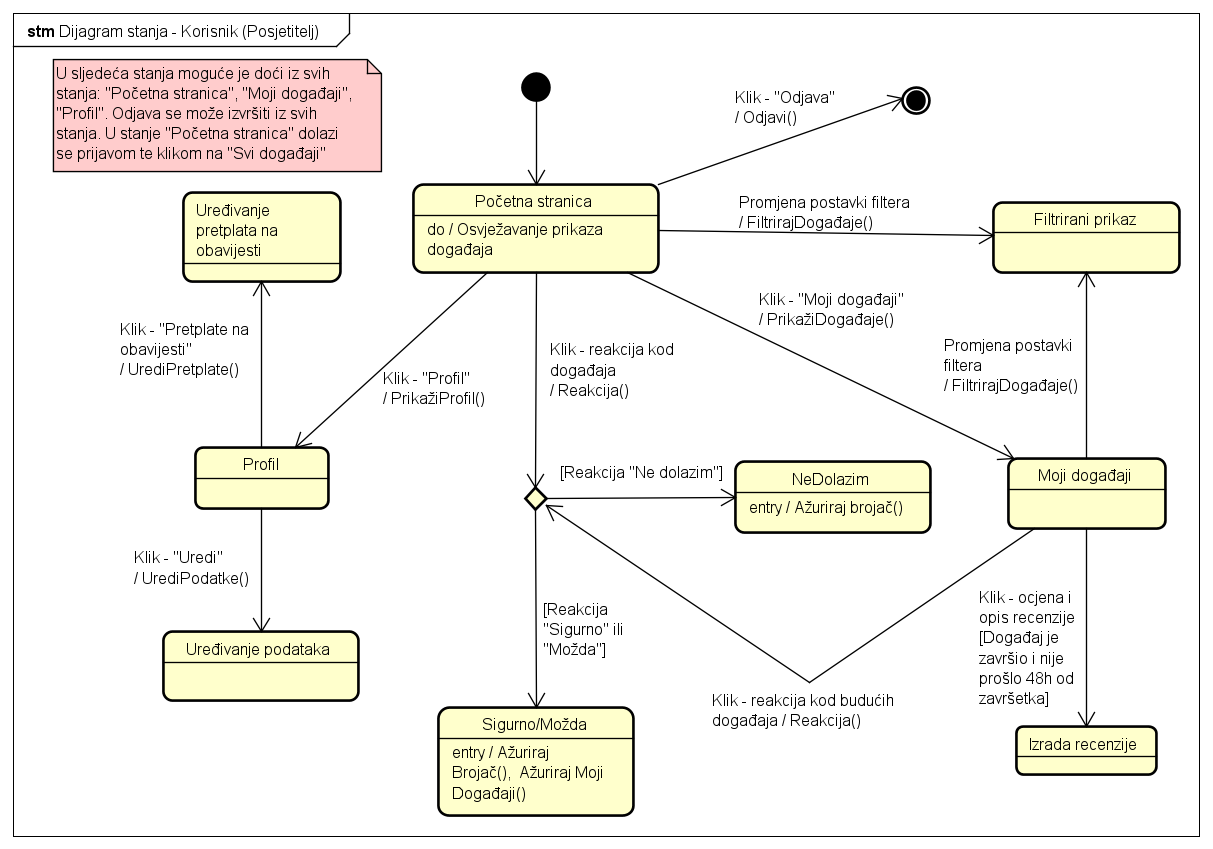
\includegraphics[scale=0.50]{dijagrami/DijagramStanja-Korisnik.png}
			\centering
			\caption{Dijagram stanja - Korisnik (Posjetitelj)}
			\label{fig:promjene}
			\end{figure}
			
			\eject 
		
		\section{Dijagram aktivnosti}
			
			Dijagram aktivnosti primjenjuje se za modeliranje poslovnih procesa, upravljačkog i podatkovnog toka. Na slici 4.8 prikazan je dijagram aktivnosti za proces stvaranje novog događaja. Nakon prijave organizator na početnoj stranici odabire opciju postavljanja događaja. Otvara mu se stranica za postavljanje događaja na kojoj unosi sve potrebne podatke o događaju. Ako organizator želi događaj bez plaćanja ulaza, podaci o događaju se odmah procesiraju, spremaju u bazu te se organizatoru prikazuje potvrda o uspješno postavljenom događaju. Ako organizator želi događaj koji će imati plaćanje ulaza, provodi se provjera članarine. Ako je članarina plaćena, proces se nastavlja jednako kao i u slučaju besplatnog događaja. Ako nije, aplikacija obavješta organizatora da članarina nije plaćena te organizator ima dvije mogućnosti: ponovno unijeti podatke o događaju i početi proces postavljanja ispočetka ili odustati od postavljanja događaja.
			
			\begin{figure}[H]
				\includegraphics[scale=0.48]{dijagrami/DijagramAktivnosti-Postavljanje_događaja.png}
				\centering
				\caption{Dijagram aktivnosti - Postavljanje događaja (Organizator)}
				\label{fig:promjene}
			\end{figure}
			
			\eject
		\section{Dijagram komponenti}
		
		Dijagram komponenti na slici opisuje organizaciju, međuovisnost komponenti i odnose prema okolini - prikazuje komponente aplikacije i glavna korištena sučelja. Korisnik pristupa aplikaciji koristeći web preglednik te preko sučelja za dohvaćanje HTML-a, CSS i JS-a poslužuje mu se frontend dio aplikacije.	REST API sučelje poslužuje podatke povezane s backend dijelom. Svaka od opisanih komponenti može imati ovisnosti prema drugim resursima, tako je backend dio povezan sa bazom podataka.
		
		\begin{figure}[H]
			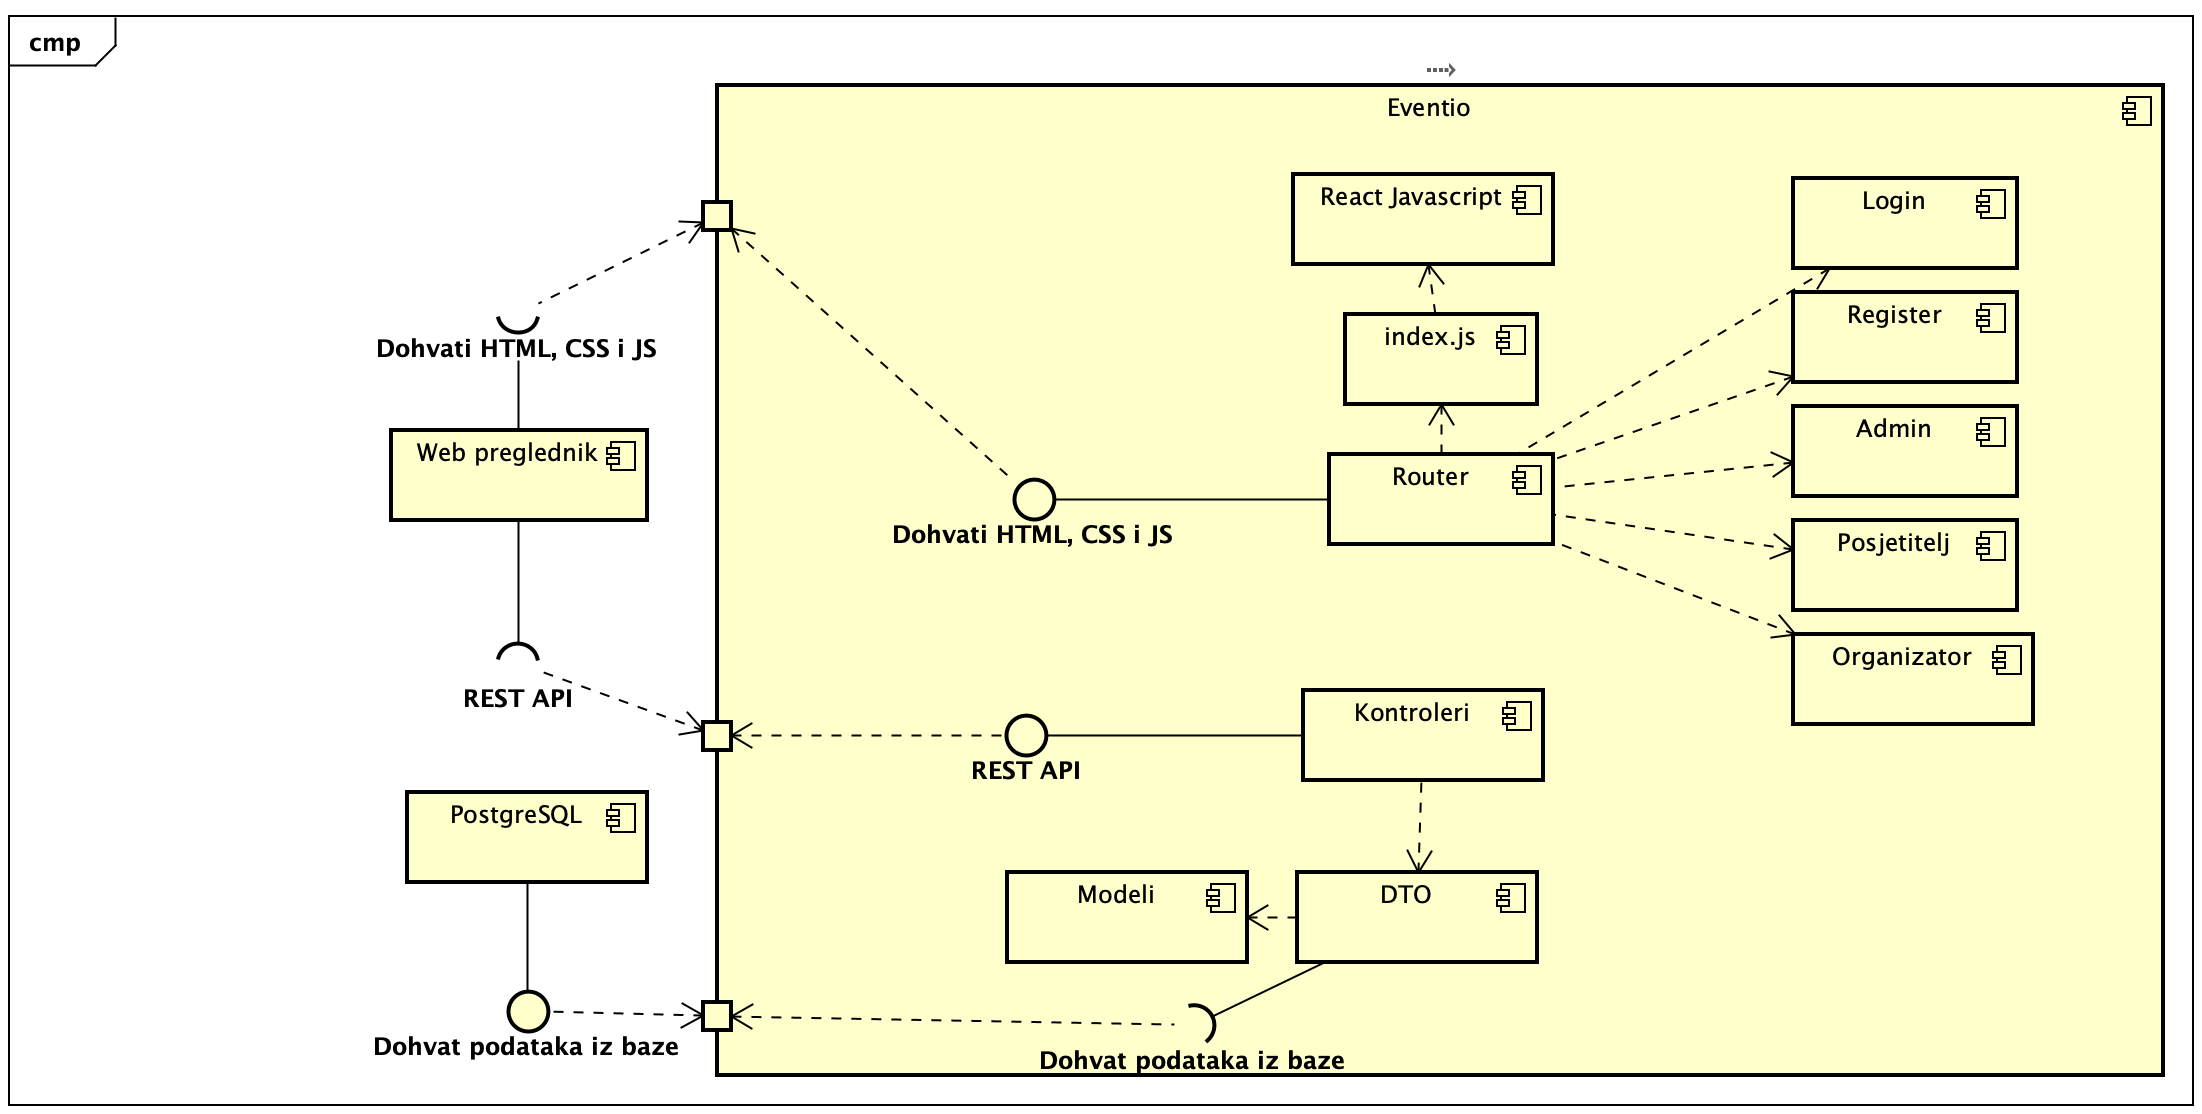
\includegraphics[scale=0.48]{dijagrami/DijagramKomponenti.png}
			\centering
			\caption{Dijagram komponenti}
			\label{fig:promjene}
		\end{figure}
	\chapter{Implementacija i korisničko sučelje}
		
		
		\section{Korištene tehnologije i alati}
		
			\textbf{\textit{dio 2. revizije}}
			
			 \textit{Detaljno navesti sve tehnologije i alate koji su primijenjeni pri izradi dokumentacije i aplikacije. Ukratko ih opisati, te navesti njihovo značenje i mjesto primjene. Za svaki navedeni alat i tehnologiju je potrebno \textbf{navesti internet poveznicu} gdje se mogu preuzeti ili više saznati o njima}.
			
			
			\eject 
		
	
		\section{Ispitivanje programskog rješenja}
			
			U ovom poglavlju usredotočili smo se na testiranje programskog rješenja testirajući cijeli sustav, ali i komponente istog. Tijekom ispitivanja komponenti sustava korišteni su JUnit za izvršavanje testova te Mockito za stvaranje mock objekata korištenih u testiranju. Selenium IDE korišten je u ispitivanju sustava te nam je omogućio brzo i precizno provjeravanje funkcionalnosti web aplikacije.
			
			\subsection{Ispitivanje komponenti}
			
			U poglavlju o ispitivanju komponenti, razvijeni su i izvršeni testovi kako bi se osigurala kvaliteta i funkcionalnost komponenata sustava, a istovremeno se time osigurava pouzdanost i održivost koda. U nastavku su prikazani primjeri nekoliko testova koji su implementirani kao dio ispitivanja komponenti sustava:

			\textbf{Test sortiranja i ispisivanja događaja} provjerava ispravnu funkcionalnost sortiranja događaja prema određenom filtru, u ovom slučaju prema vremenu početka događaja. Također testirano je izlistavanje događaja, je li broj događaja jednak očekivanom broju. Korišten je JUnit za pisanje i izvršavanje testova te Mockito za stvaranje mock objekta i postavljanje očekivanja.


			\textbf{Test registracije korisinika} ispituje uspješnost registracije korisnika. Također se koriste Mock objekti koji simuliraju ponašanje komponenti tijekom registracije. Prikazana su dva testa, u jednom se testira registracija koja je uspješa, u drugom se testira neuspješna registracija korisnika.

			U nastavku su još prikazani sljedeći testovi: \textbf{Test slanja e-maila}, \textbf{Test spremanja recenzije}, \textbf{Test spremanja zainteresiranosti}. Oni redom provjeravaju točnost slanja e-maila, ispravnu funkcionalnost spremanja recenzije i zainteresiranosti. U navedenim testovima se također koriste spomenute tehnologije za provjeravanje ispravnosti. Osim testova, prikazano je i njihovo izvođenje te rezultat izvođenja.
			
			\begin{figure}[H]
				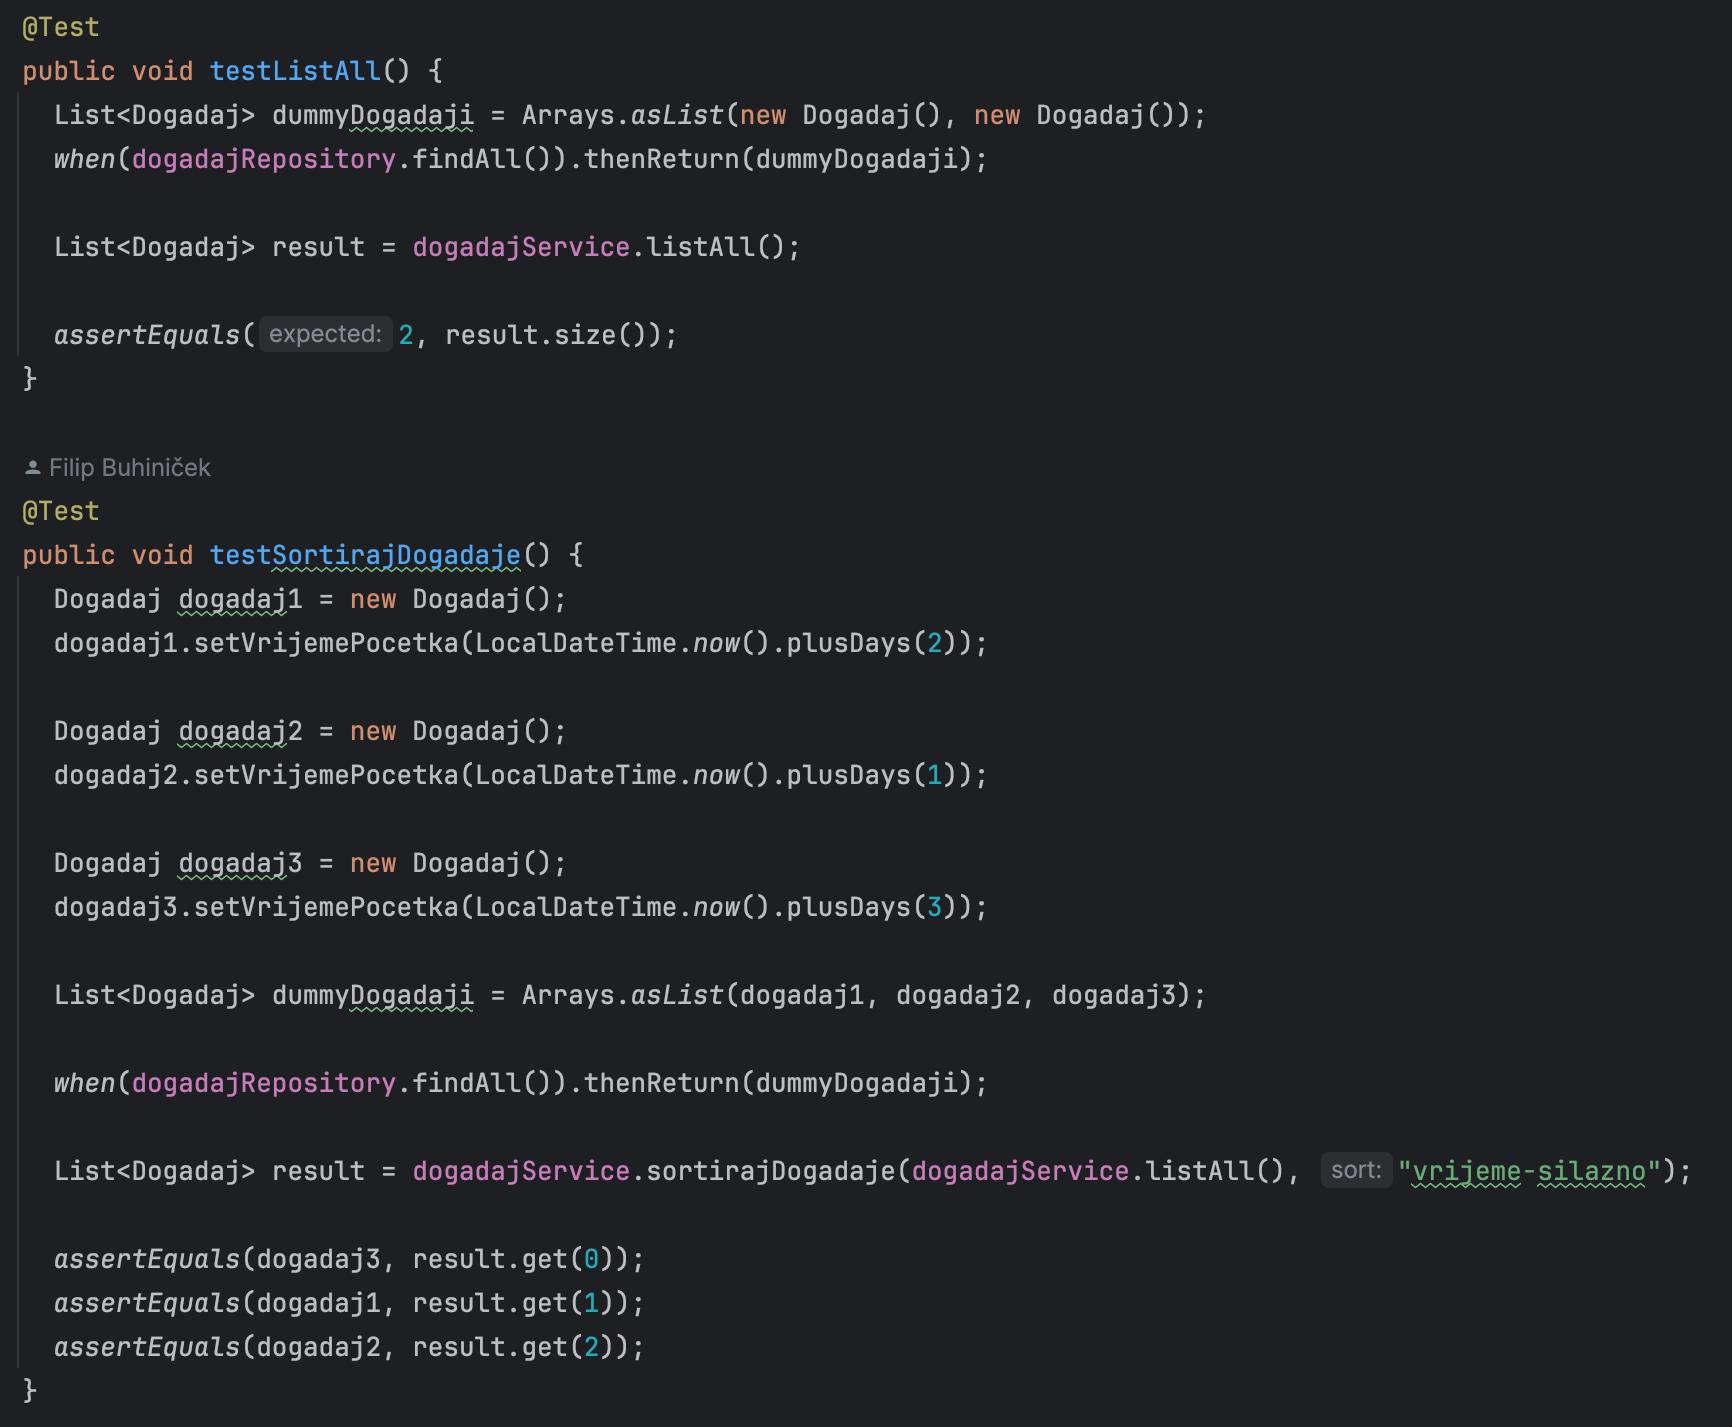
\includegraphics[scale=0.45]{testovi/dogadajTest.png}
				\centering
				\caption{Test za sortiranje i ispisivanje događaja}
				\label{fig:promjene}
			\end{figure}
			
			
			\begin{figure}[H]
				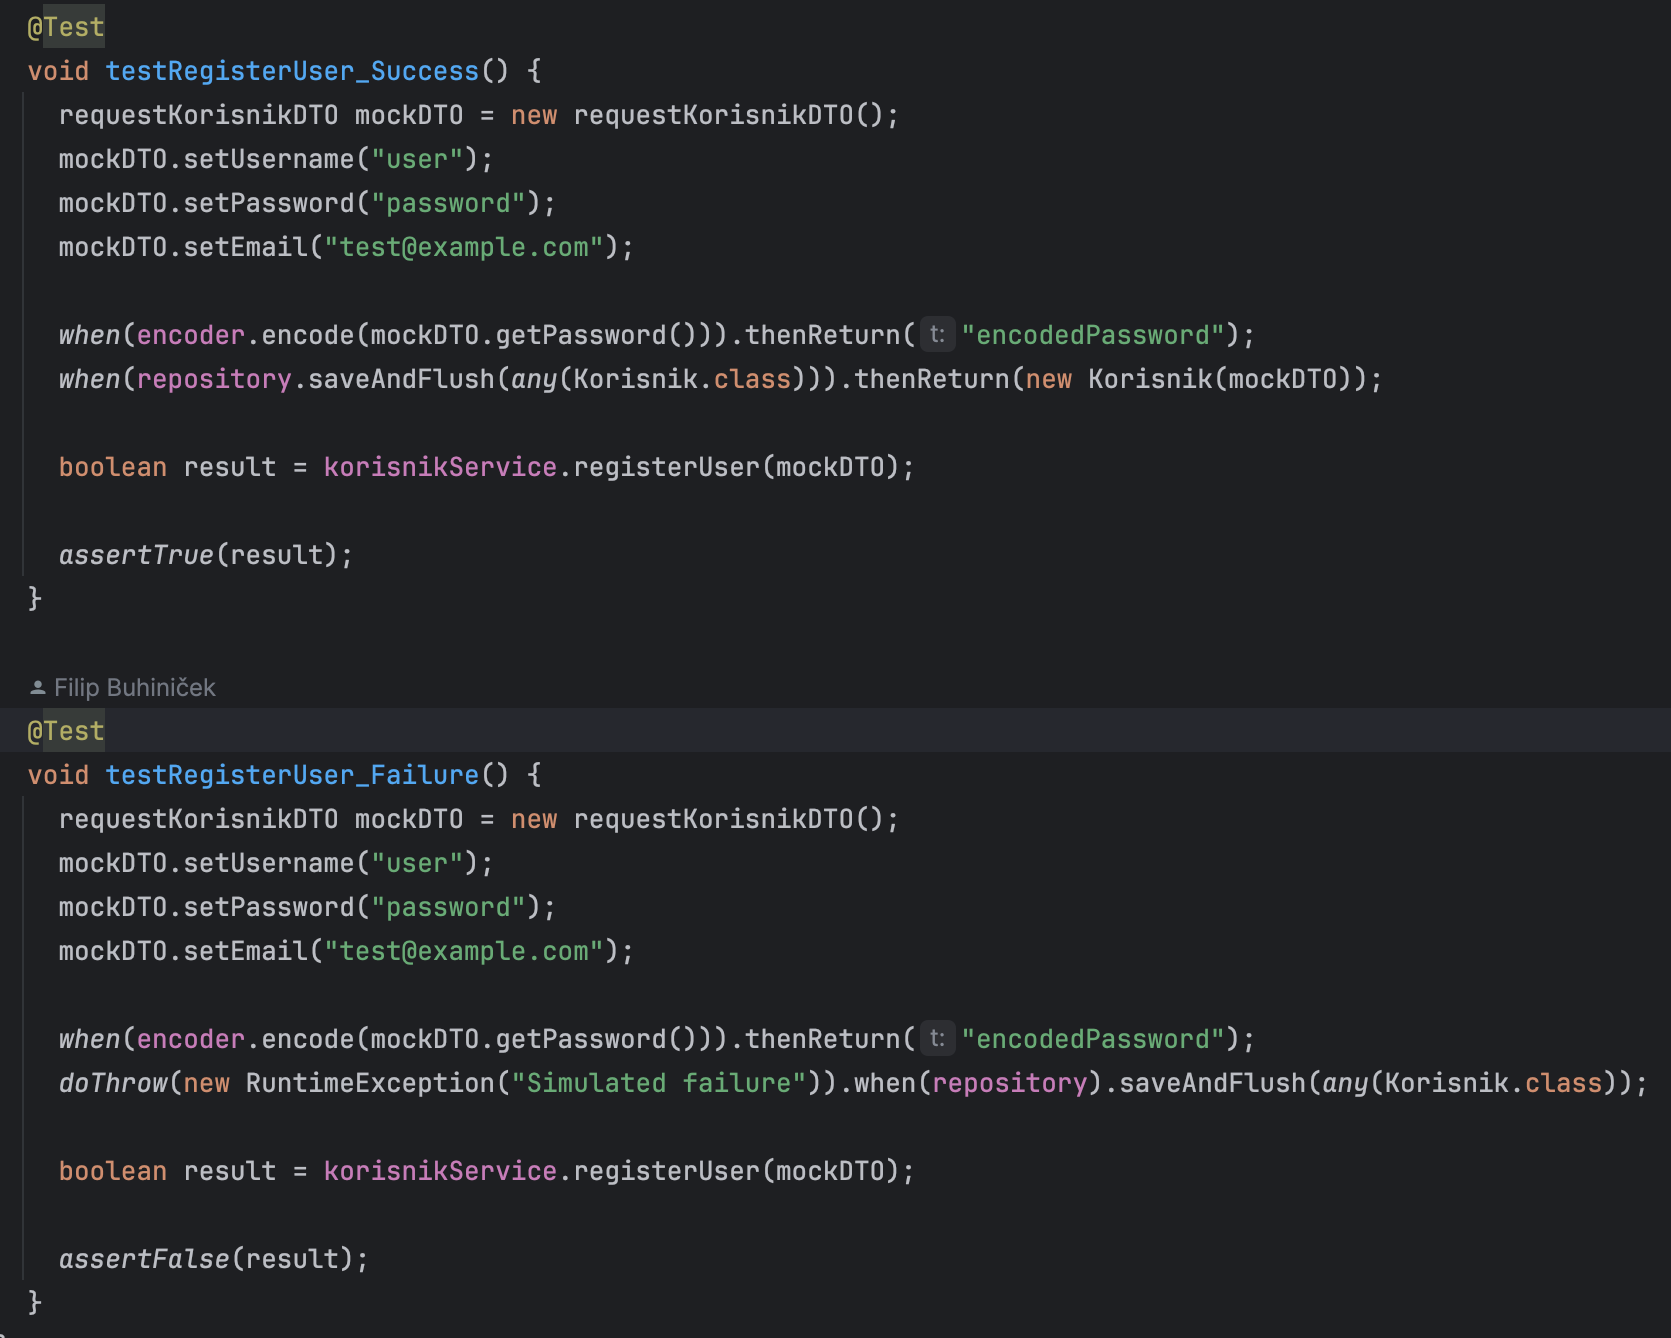
\includegraphics[scale=0.45]{testovi/korisnikTest.png}
				\centering
				\caption{Test registracije korisnika}
				\label{fig:promjene}
			\end{figure}
			
			
			
			\begin{figure}[H]
				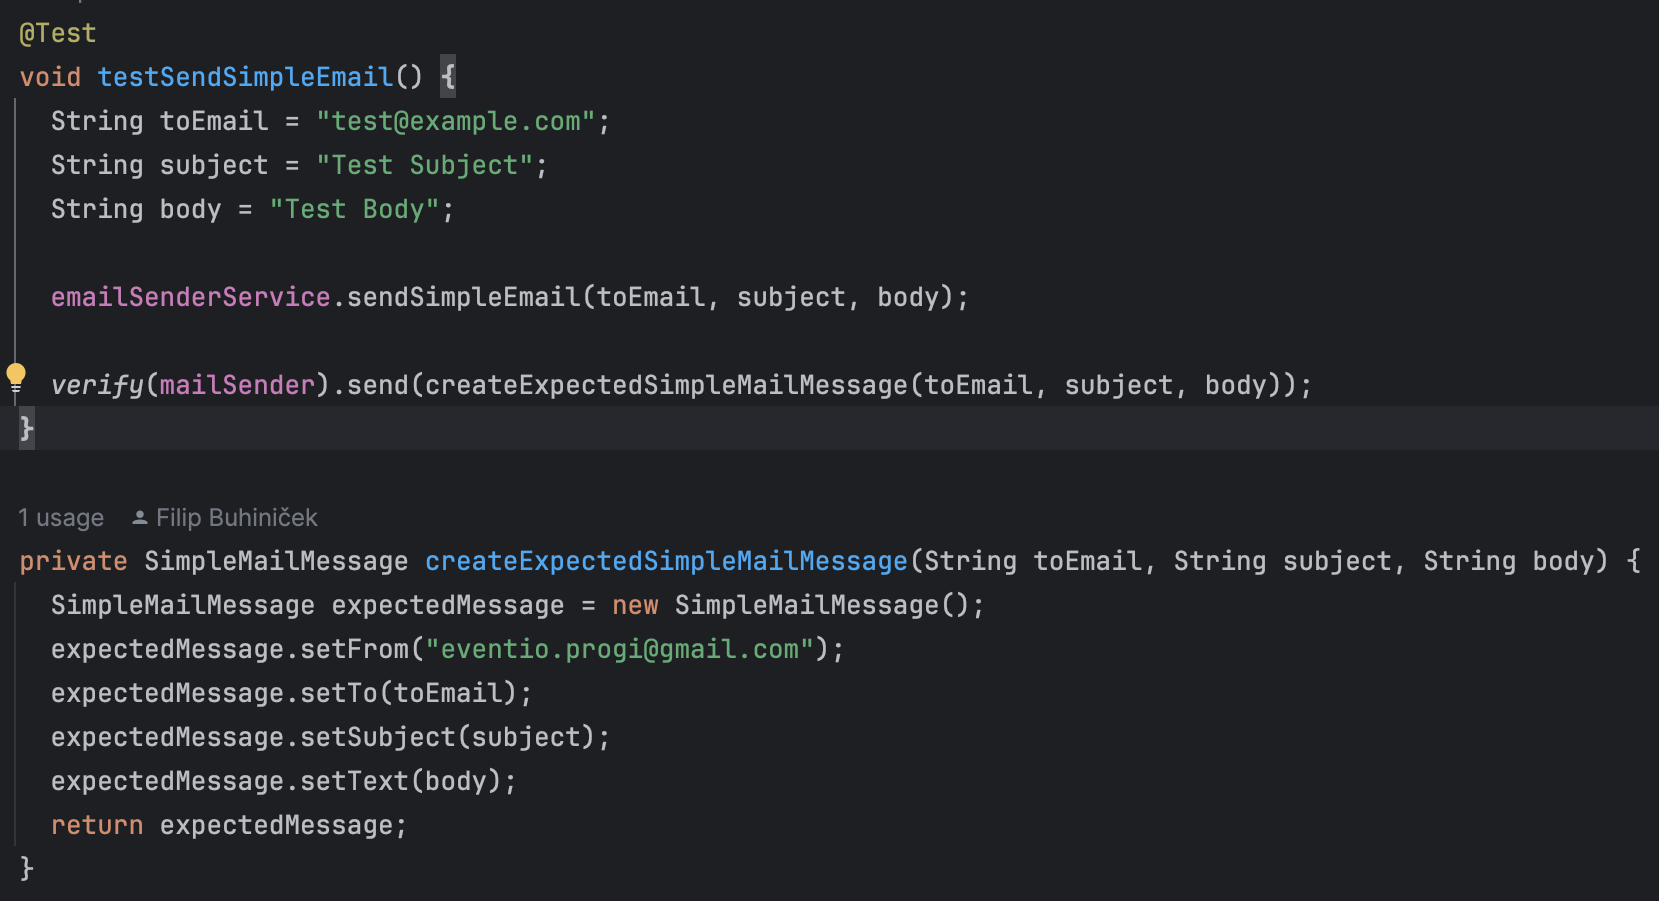
\includegraphics[scale=0.45]{testovi/emailTest.png}
				\centering
				\caption{Test slanja e-maila}
				\label{fig:promjene}
			\end{figure}
			
			\begin{figure}[H]
				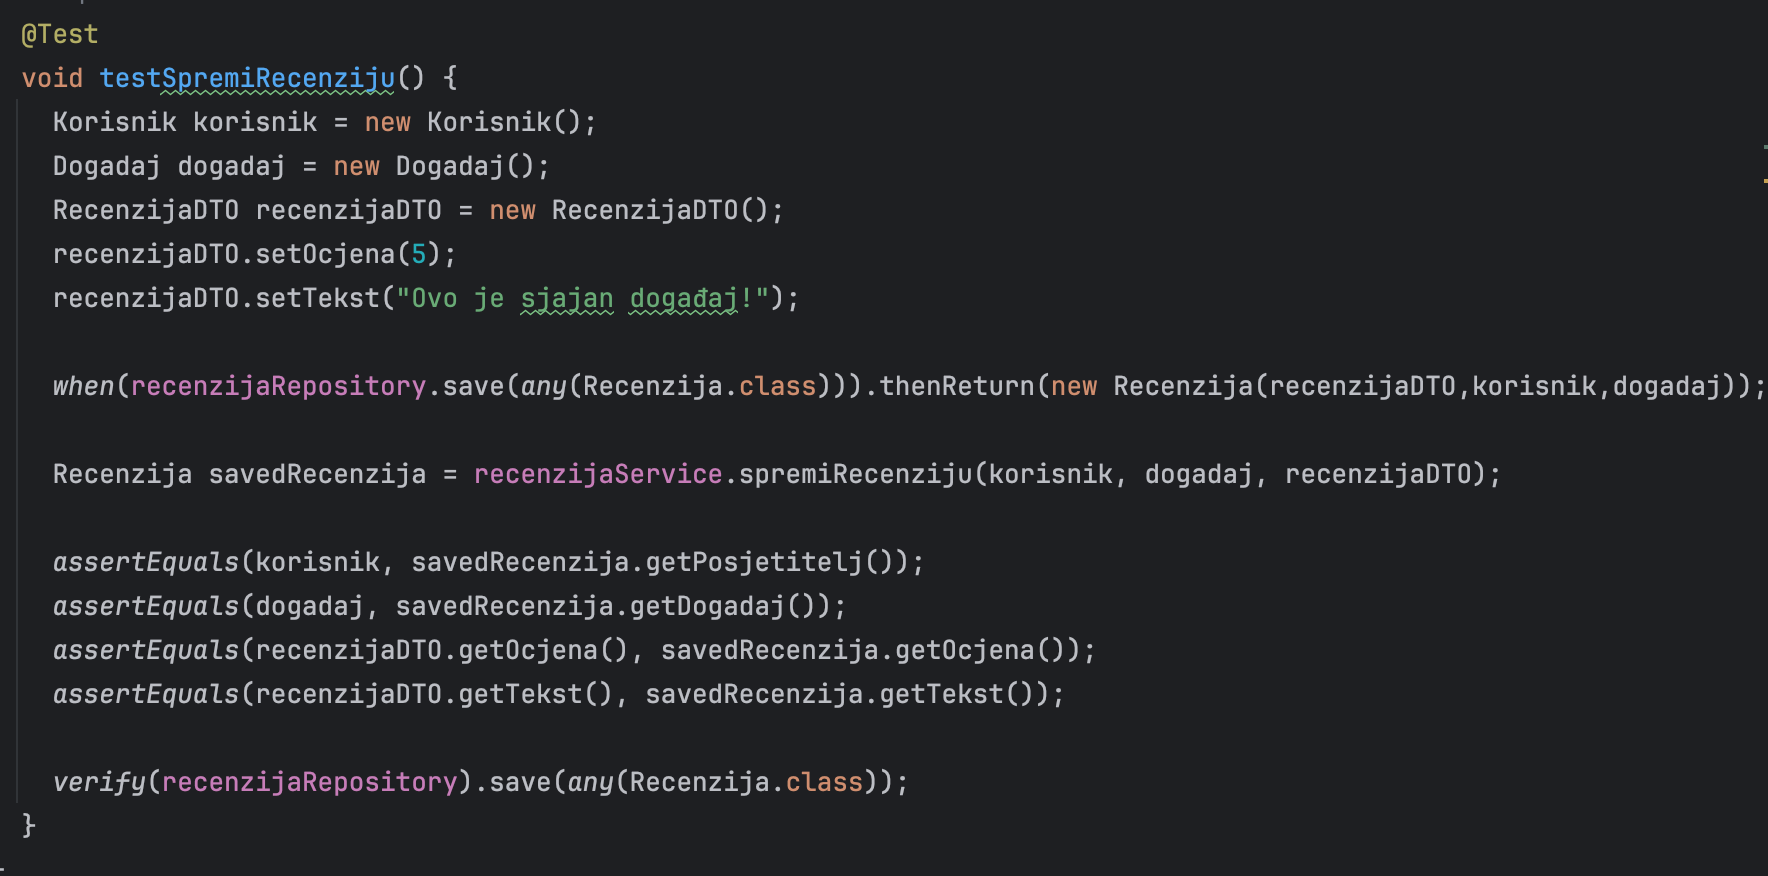
\includegraphics[scale=0.45]{testovi/recenzijeTest.png}
				\centering
				\caption{Test spremanja recenzije}
				\label{fig:promjene}
			\end{figure}
			
			\begin{figure}[H]
				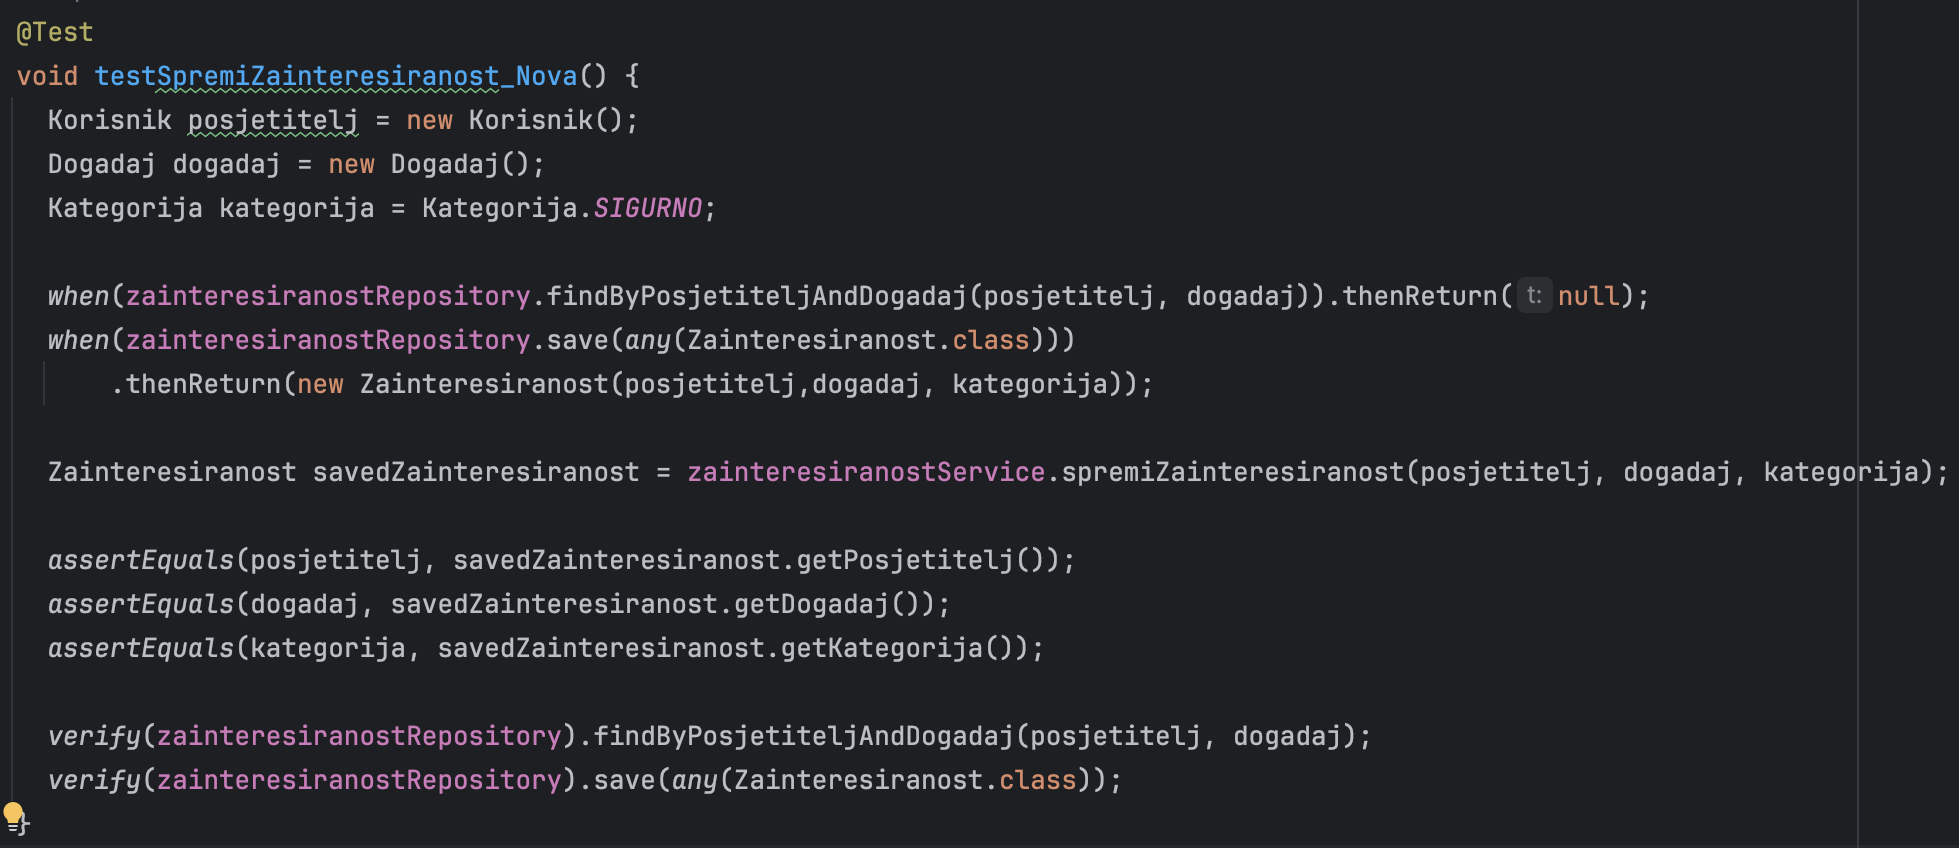
\includegraphics[scale=0.45]{testovi/zainteresiranostTest1.png}
				\centering
				\caption{Test spremanja nove zainteresiranosti}
				\label{fig:promjene}
			\end{figure}
			
			\begin{figure}[H]
				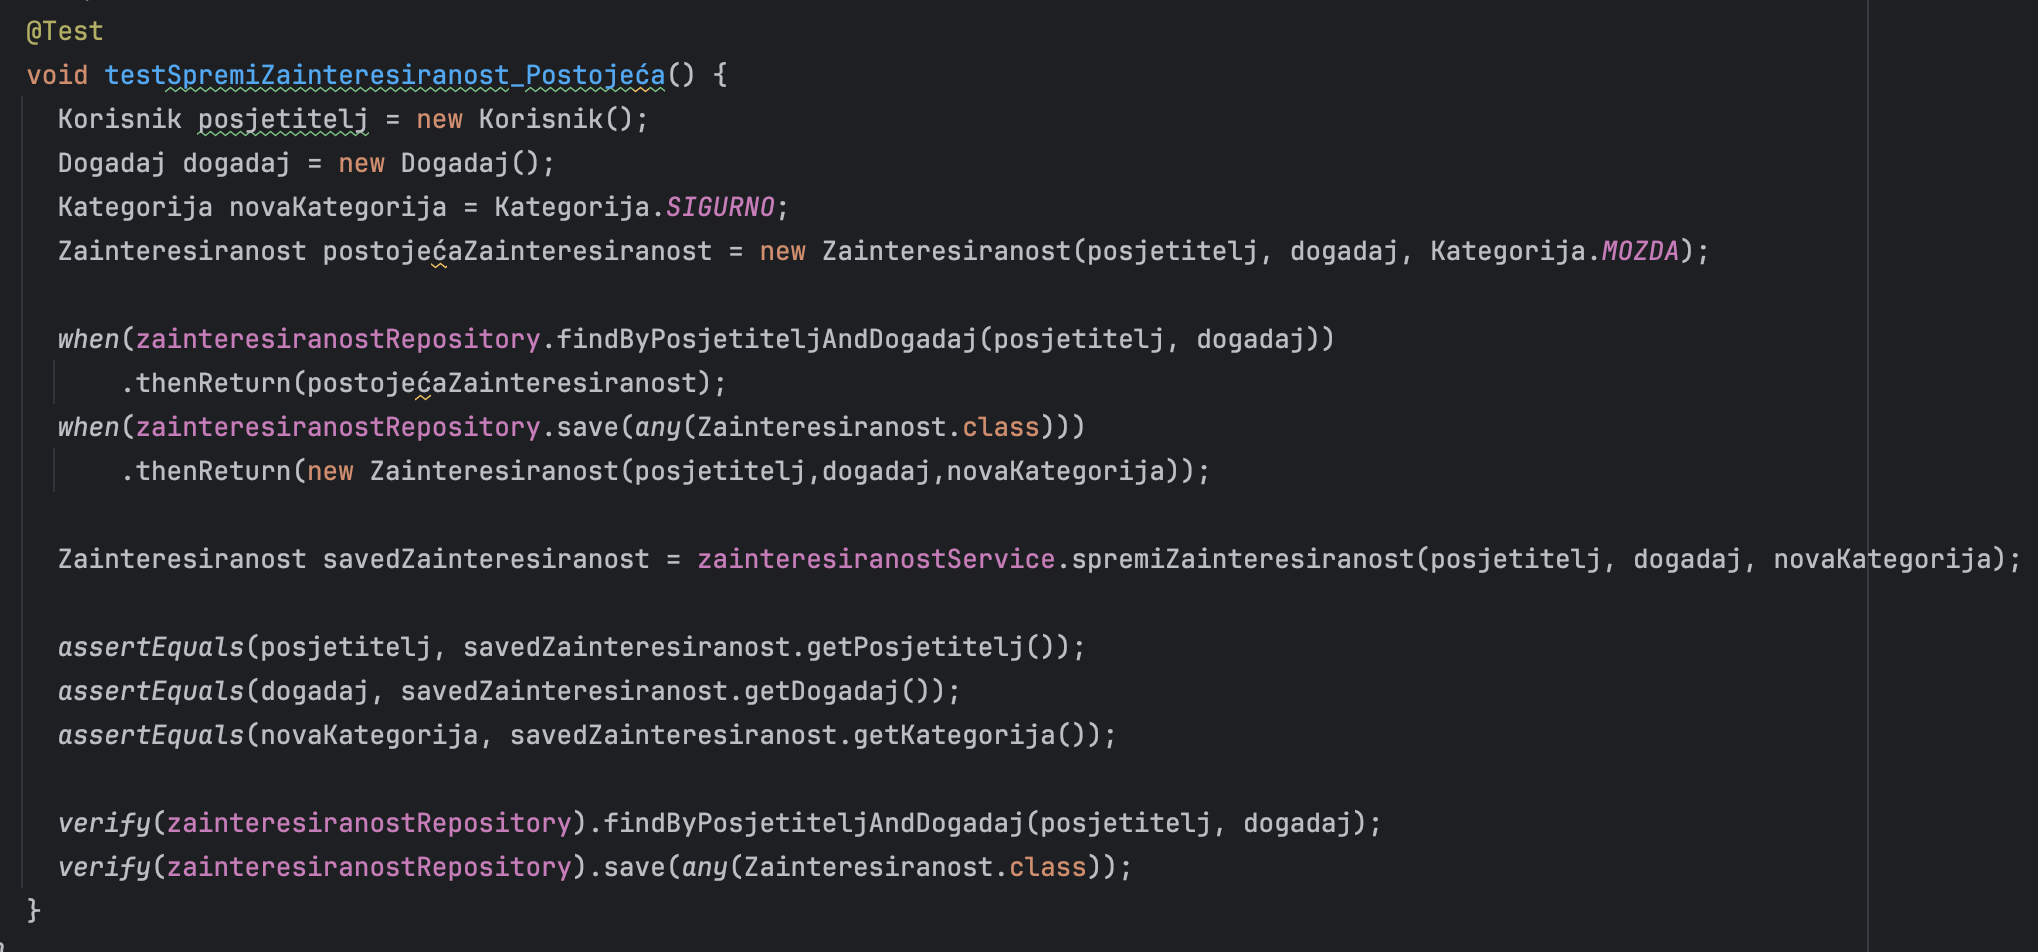
\includegraphics[scale=0.45]{testovi/zainteresiranostTest2.png}
				\centering
				\caption{Test spremanja postojeće zainteresiranosti}
				\label{fig:promjene}
			\end{figure}
			
				\begin{figure}[H]
				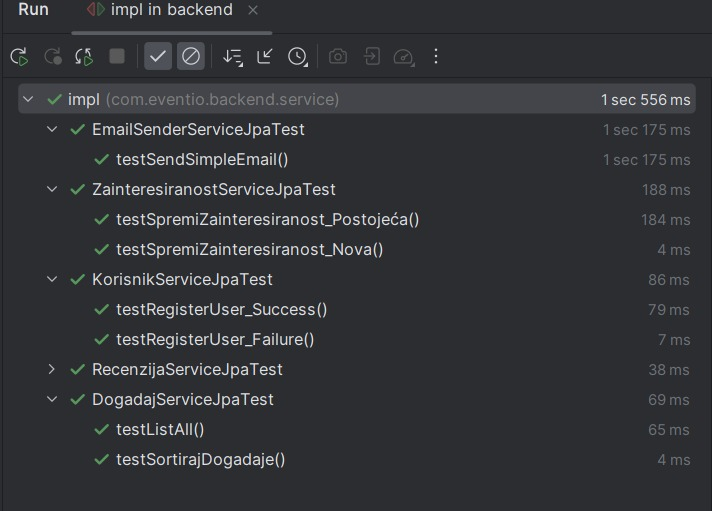
\includegraphics[scale=0.45]{testovi/unit_testovi.jpeg}
				\centering
				\caption{Izvršavanje i rezultati testova}
				\label{fig:promjene}
			\end{figure}
			
			
			\subsection{Ispitivanje sustava}
			
			U procesu ispitivanja sustava koristili smo Selenium IDE koji nam je omogućio precizno i brzo testiranje funkcionalnosti web aplikacije. Selenium IDE predstavlja moćan alat za testiranje web aplikacija te se istovremeno olakšava proces automatizacije. \newline Na sljedećim slikama prikazani su ispitni slučajevima kojima smo testirali funkcionalnost aplikacije. \textbf{Test prijave organizatora} provjerava uspješnost prijave korisnika koji je organizator. \textbf{Test stvaranja novog događaja} provjerava funkcionalnost stvaranja novog događaja sa svim postavkama. Prikazano je i izvršavanje \textbf{Testa promjene cijene pretplate} i \textbf{Testa stvaranja nove recenzije}.
			
			\begin{figure}[H]
				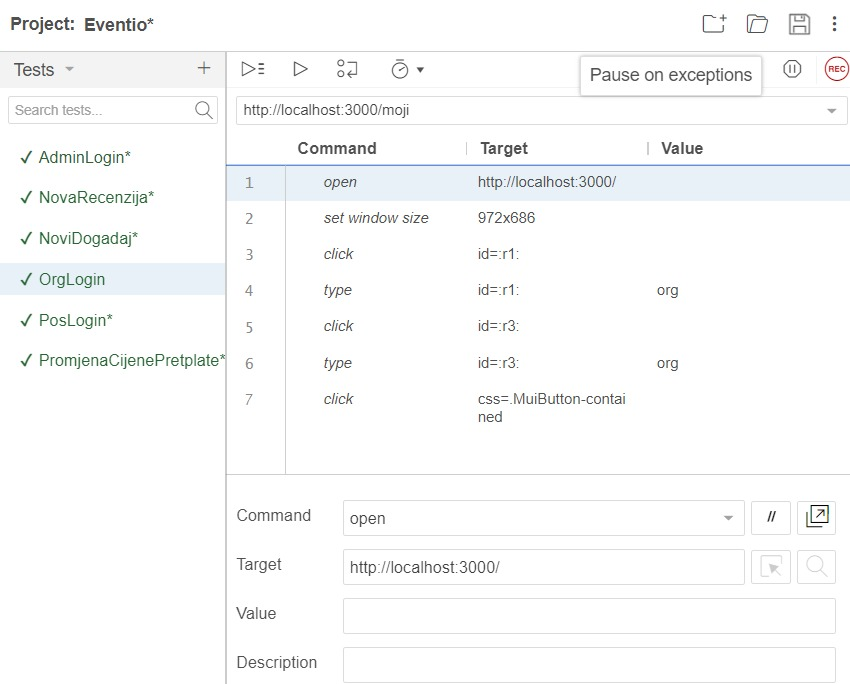
\includegraphics[scale=0.45]{testovi/selOrgLogin.jpeg}
				\centering
				\caption{Test prijave organizatora}
				\label{fig:promjene}
			\end{figure}
			
			\begin{figure}[H]
				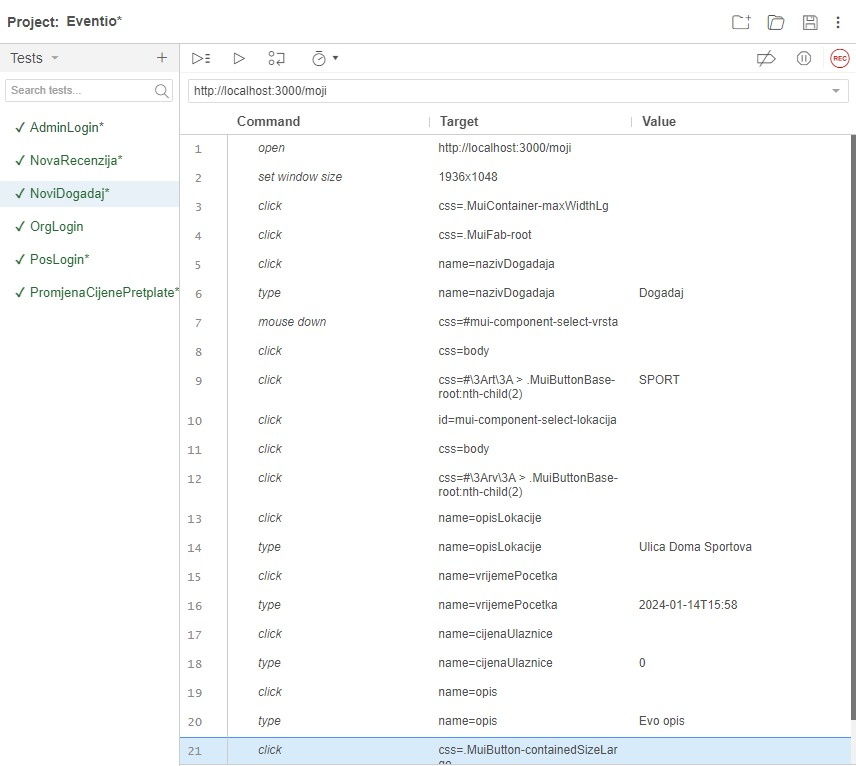
\includegraphics[scale=0.45]{testovi/selNoviDogadaj.jpeg}
				\centering
				\caption{Test stvaranja novog događaja}
				\label{fig:promjene}
			\end{figure}
			
			\begin{figure}[H]
				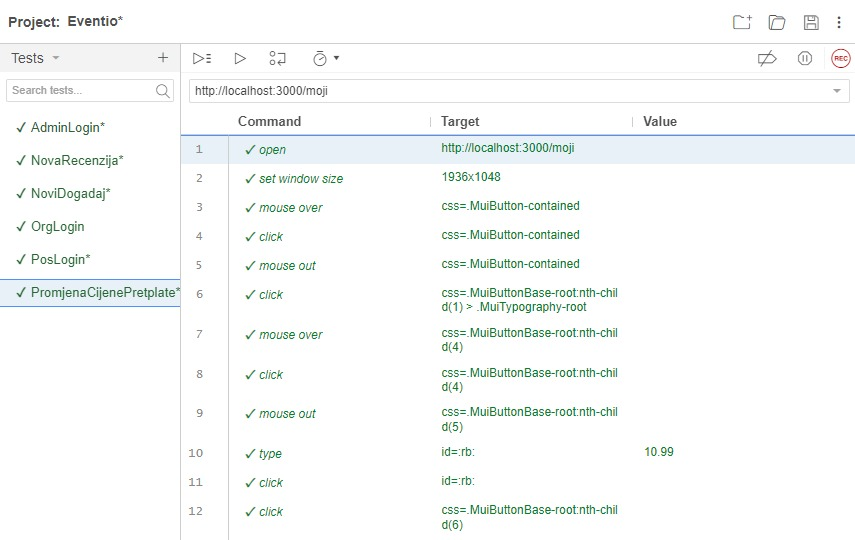
\includegraphics[scale=0.45]{testovi/selPretplata.jpeg}
				\centering
				\caption{Test promjena cijene pretplate}
				\label{fig:promjene}
			\end{figure}
			
			\begin{figure}[H]
				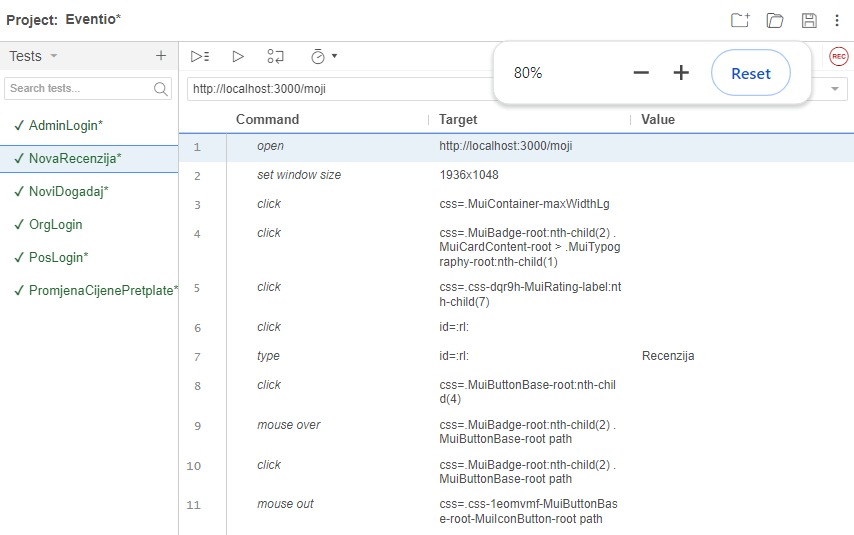
\includegraphics[scale=0.45]{testovi/selRecenzija.jpeg}
				\centering
				\caption{Test stvaranje nove recenzije}
				\label{fig:promjene}
			\end{figure}
			
		
		
		\section{Dijagram razmještaja}
			
			Dijagrami razmještaja opisuju topologiju sklopovlja i programsku potporu koja se koristi u implementaciji sustava u njegovom radnom okruženju. Korisnici pristupaju web aplikaciji putem web preglednika na svojim osobnim računalima. Arhitektura sustava temelji se na jasno odvojenim slojevima: frontendu, backendu i bazi podataka. 
			Frontend poslužitelj posvećen je izvršavanju i posluživanju resursa vezanih uz korisničko sučelje. Backend poslužitelj fokusiran  je na izvršavanje poslovne logike, pružanje API-ja te komunikaciju s bazom podataka. Na ovom sloju obavljaju se operacije i logika sustava, pružajući funkcionalnosti koje podržavaju rad aplikacije. Baza podataka poslužitelj je posvećen upravljanju bazom podataka. Ovdje se nalazi sama baza podataka i sustav za pohranu i dohvat podataka.  Komunikacija između korisnika i poslužitelja odvija se preko HTTP veze.
			 
			 \begin{figure}[H]
			 	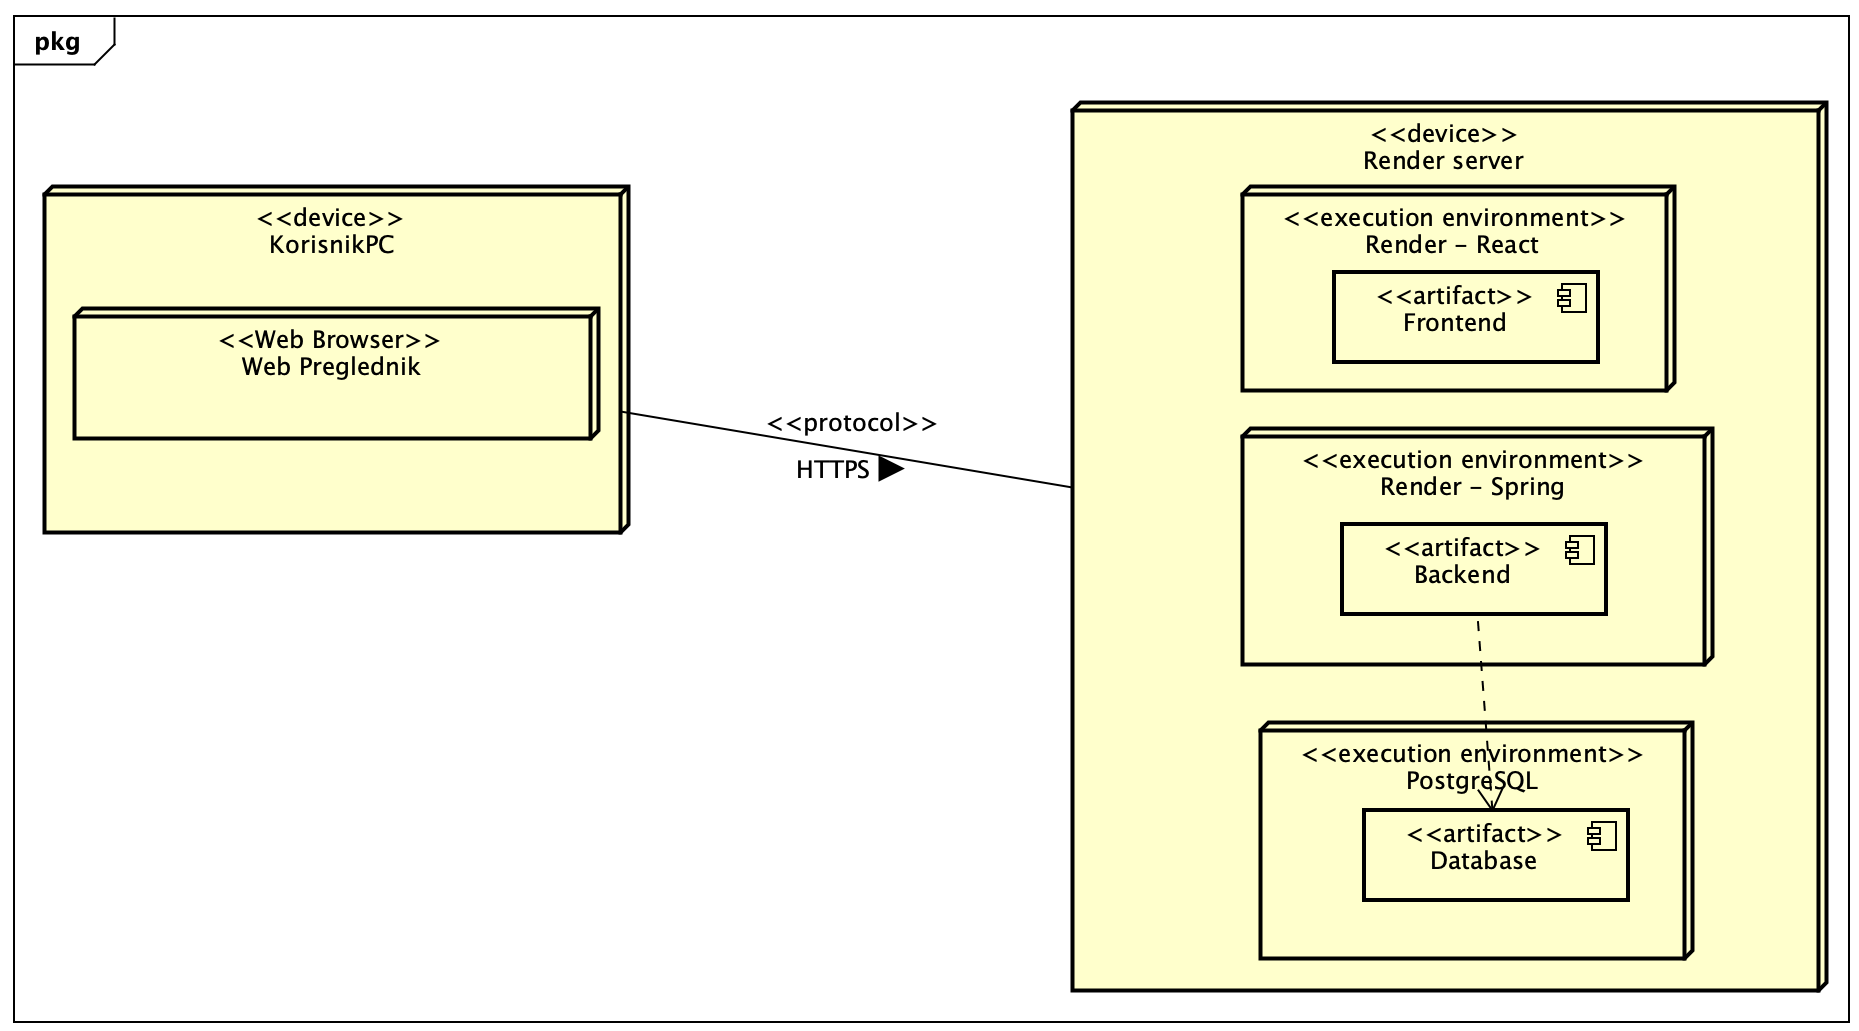
\includegraphics[scale=0.45]{dijagrami/dijagramRazmjestaja.png}
			 	\centering
			 	\caption{Dijagram razmještaja}
			 	\label{fig:promjene}
			 \end{figure}
			
			\eject 
		
		\section{Upute za puštanje u pogon}
		
			\textbf{\textit{dio 2. revizije}}\\
		
			 \textit{U ovom poglavlju potrebno je dati upute za puštanje u pogon (engl. deployment) ostvarene aplikacije. Na primjer, za web aplikacije, opisati postupak kojim se od izvornog kôda dolazi do potpuno postavljene baze podataka i poslužitelja koji odgovara na upite korisnika. Za mobilnu aplikaciju, postupak kojim se aplikacija izgradi, te postavi na neku od trgovina. Za stolnu (engl. desktop) aplikaciju, postupak kojim se aplikacija instalira na računalo. Ukoliko mobilne i stolne aplikacije komuniciraju s poslužiteljem i/ili bazom podataka, opisati i postupak njihovog postavljanja. Pri izradi uputa preporučuje se \textbf{naglasiti korake instalacije uporabom natuknica} te koristiti što je više moguće \textbf{slike ekrana} (engl. screenshots) kako bi upute bile jasne i jednostavne za slijediti.}
			
			
			 \textit{Dovršenu aplikaciju potrebno je pokrenuti na javno dostupnom poslužitelju. Studentima se preporuča korištenje neke od sljedećih besplatnih usluga: \href{https://aws.amazon.com/}{Amazon AWS}, \href{https://azure.microsoft.com/en-us/}{Microsoft Azure} ili \href{https://www.heroku.com/}{Heroku}. Mobilne aplikacije trebaju biti objavljene na F-Droid, Google Play ili Amazon App trgovini.}
			
			
			\eject 
	\chapter{Zaključak i budući rad}
		
		Cilj našeg projekta bio je razviti programsku podršku za web aplikaciju "Eventio", inovativnu platformu za promociju zabavnih događanja u gradu, koja bi korisnicima omogućila jednostavno stvaranje i sudjelovanje na događanjima. Ova inovativna web aplikacija je koncipirana kako bi korisnicima pružila laksi pristup društvenim događanjima koja odgovaraju njihovim interesima, istovremeno olakšavajući organizaciju i promociju tih događanja.
		
		Formiran je tim od sedam članova koji su u razdoblju od 17 tjedana surađivali na ovom projektu. Za svakodnevnu komunikaciju koristili smo WhatsApp, Discord za održavanje remote sastanaka, te česte timske sastanke uživo kako bismo zajedno raspravljali o tijeku projekta, izazovima, i mogućim unapređenjima. Razvili smo internu raspodjelu zadataka koji su bili podijeljeni članovima tima što je osiguralo konstantan rad na projektu. Tome je pomogla i interna struktura tima podijeljena podijeljena u podtimove s većim fokusom na drukčijim dijelovima projekta, uključujući backend, frontend i dokumentaciju. Iskusniji članovi su pružali mentorstvo i podršku onima s manje iskustva, olakšavajući im savladavanje novih tehnologija i koncepta.
		
		Prva faza projekta, počevši s okupljanjem tima, bila je ključna za razvoj međusobnih odnosa, što je rezultiralo učinkovitijom suradnjom u kasnijim fazama. Osim toga, faza je obuhvatila rad na dokumentaciji, uključujući izradu obrazaca uporabe, sekvencijske dijagrame, model baze podataka, dijagrame razreda. Izrada navedenih dijagrama, ali i vizualnih rješenja programskog zadatka bile su od ključne važnosti za usmjeravanje razvoja te su uvelike olakšale implementaciju rješenja.
		
		Druga faza projekta bila je usmjerena na konkretan razvoj web aplikacije. Osim samog programiranja, ova faza uključivala je detaljno dokumentiranje projekta, uključujući UML dijagrame (dijagram stanja, aktivnosti, komponenti i razmještaja) te izradu popratne dokumentacije koja je obuhvatila opis testiranja, deployment procese i druge važne aspekte implementacije.
		
		Gledajući prema budućnosti, projekt pruža niz mogućnosti za daljnje unapređenje. Jedna od mogućnosti je razvoj mobilne aplikacije kako bi se omogućilo korisnicima pristup događanjima putem mobilnih uređaja. Također, smatramo da bi uvođenje sustava za chat na događanjima dodatno obogatilo korisničko iskustvo omogućavajući sudionicima međusobnu komunikaciju. Osim toga, daljnje širenje na područja izvan Zagreba, primjerice na razini Republike Hrvatske, predstavlja logičan korak u razvoju projekta.
		
		Iskustvo rada na ovom projektu bilo je izuzetno korisno za sve članove tima. Poboljšali smo ne samo tehničke vještine već i sposobnosti komunikacije, planiranja i timskog rada. Sudjelovanje u projektu pružilo nam je uvid u dinamiku rada u timu te nas pripremilo za buduće izazove u našim karijerama. Zadovoljni smo rezultatom ovog projekta i što smo bili njegov dio te se veselimo nastavku učenja i rasta u budućnosti.
		
		\eject 
	\chapter*{Popis literature}
		\addcontentsline{toc}{chapter}{Popis literature}
	 	
 		\textbf{\textit{Kontinuirano osvježavanje}}
	
		\textit{Popisati sve reference i literaturu koja je pomogla pri ostvarivanju projekta.}
		
		
		\begin{enumerate}
			
			
			\item  Programsko inženjerstvo, FER ZEMRIS, \url{http://www.fer.hr/predmet/proinz}
			
			\item  I. Sommerville, "Software engineering", 8th ed, Addison Wesley, 2007.
			
			\item  T.C.Lethbridge, R.Langaniere, "Object-Oriented Software Engineering", 2nd ed. McGraw-Hill, 2005.
			
			\item  I. Marsic, Software engineering book``, Department of Electrical and Computer Engineering, Rutgers University, \url{http://www.ece.rutgers.edu/~marsic/books/SE}
			
			\item  The Unified Modeling Language, \url{https://www.uml-diagrams.org/}
			
			\item  Astah Community, \url{http://astah.net/editions/uml-new}
		\end{enumerate}
		
		 
	
	
	\begingroup
	\renewcommand*\listfigurename{Indeks slika i dijagrama}
	%\renewcommand*\listtablename{Indeks tablica}
	%\let\clearpage\relax
	\listoffigures
	%\vspace{10mm}
	%\listoftables
	\endgroup
	\addcontentsline{toc}{chapter}{Indeks slika i dijagrama}


	
	\eject 
		
	\chapter*{Dodatak: Prikaz aktivnosti grupe}
		\addcontentsline{toc}{chapter}{Dodatak: Prikaz aktivnosti grupe}
		
		\section*{Dnevnik sastajanja}
		
		\textbf{\textit{Kontinuirano osvježavanje}}\\
		
		 \textit{U ovom dijelu potrebno je redovito osvježavati dnevnik sastajanja prema predlošku.}
		
		\begin{packed_enum}
			\item  sastanak
			
			\item[] \begin{packed_item}
				\item Datum: u ovom formatu: \today
				\item Prisustvovali: I.Prezime, I.Prezime
				\item Teme sastanka:
				\begin{packed_item}
					\item  opis prve teme
					\item  opis druge teme
				\end{packed_item}
			\end{packed_item}
			
			\item  sastanak
			\item[] \begin{packed_item}
				\item Datum: u ovom formatu: \today
				\item Prisustvovali: I.Prezime, I.Prezime
				\item Teme sastanka:
				\begin{packed_item}
					\item  opis prve teme
					\item  opis druge teme
				\end{packed_item}
			\end{packed_item}
			
			%
			
		\end{packed_enum}
		
		\eject
		\section*{Tablica aktivnosti}
		
			\textbf{\textit{Kontinuirano osvježavanje}}\\
			
			 \textit{Napomena: Doprinose u aktivnostima treba navesti u satima po članovima grupe po aktivnosti.}

			\begin{longtblr}[
					label=none,
				]{
					vlines,hlines,
					width = \textwidth,
					colspec={X[7, l]X[1, c]X[1, c]X[1, c]X[1, c]X[1, c]X[1, c]X[1, c]}, 
					vline{1} = {1}{text=\clap{}},
					hline{1} = {1}{text=\clap{}},
					rowhead = 1,
				} 
			
				\SetCell[c=1]{c}{} & \SetCell[c=1]{c}{\rotatebox{90}{\textbf{Gašpar Haramija}}} & \SetCell[c=1]{c}{\rotatebox{90}{\textbf{Filip Buhiniček}}} &	\SetCell[c=1]{c}{\rotatebox{90}{\textbf{Sandro Boka}}} & \SetCell[c=1]{c}{\rotatebox{90}{\textbf{Marko Sršić }}} &	\SetCell[c=1]{c}{\rotatebox{90}{\textbf{Mateo Grdić}}} & \SetCell[c=1]{c}{\rotatebox{90}{\textbf{Nikola Kušen}}} &	\SetCell[c=1]{c}{\rotatebox{90}{\textbf{Ime Prezime }}} \\  
				Upravljanje projektom 		&  &  &  &  &  &  & \\ 
				Opis projektnog zadatka 	&  &  &  &  &  &  & \\ 
				
				Funkcionalni zahtjevi       &  &  &  &  &  &  &  \\ 
				Opis pojedinih obrazaca 	&  &  &  &  &  &  &  \\ 
				Dijagram obrazaca 			&  &  &  &  &  &  &  \\ 
				Sekvencijski dijagrami 		&  &  &  &  &  &  &  \\ 
				Opis ostalih zahtjeva 		&  &  &  &  &  &  &  \\ 

				Arhitektura i dizajn sustava	 &  &  &  &  &  &  &  \\ 
				Baza podataka				&  &  &  &  &  &  &   \\ 
				Dijagram razreda 			&  &  &  &  &  &  &   \\ 
				Dijagram stanja				&  &  &  &  &  &  &  \\ 
				Dijagram aktivnosti 		&  &  &  &  &  &  &  \\ 
				Dijagram komponenti			&  &  &  &  &  &  &  \\ 
				Korištene tehnologije i alati 		&  &  &  &  &  &  &  \\ 
				Ispitivanje programskog rješenja 	&  &  &  &  &  &  &  \\ 
				Dijagram razmještaja			&  &  &  &  &  &  &  \\ 
				Upute za puštanje u pogon 		&  &  &  &  &  &  &  \\  
				Dnevnik sastajanja 			&  &  &  &  &  &  &  \\ 
				Zaključak i budući rad 		&  &  &  &  &  &  &  \\  
				Popis literature 			&  &  &  &  &  &  &  \\  
				&  &  &  &  &  &  &  \\ \hline 
				\textit{Dodatne stavke kako ste podijelili izradu aplikacije} 			&  &  &  &  &  &  &  \\ 
				\textit{npr. izrada početne stranice} 				&  &  &  &  &  &  &  \\  
				\textit{izrada baze podataka} 		 			&  &  &  &  &  &  & \\  
				\textit{spajanje s bazom podataka} 							&  &  &  &  &  &  &  \\ 
				\textit{back end} 							&  &  &  &  &  &  &  \\  
				 							&  &  &  &  &  &  &\\ 
			\end{longtblr}
					
					
		\eject
		\section*{Dijagrami pregleda promjena}
		
		\textbf{\textit{dio 2. revizije}}\\
		
		\textit{Prenijeti dijagram pregleda promjena nad datotekama projekta. Potrebno je na kraju projekta generirane grafove s gitlaba prenijeti u ovo poglavlje dokumentacije. Dijagrami za vlastiti projekt se mogu preuzeti s gitlab.com stranice, u izborniku Repository, pritiskom na stavku Contributors.}
		
	


\end{document} %naredbe i tekst nakon ove naredbe ne ulaze u izgrađen dokument 


